%!TEX program = xelatex%
%!BIB program = biber%
% 出现任何问题请联系(zhangxinhang19@foxmial.com)
\documentclass[biber,ttf]{nudtpaper}
% biber-参考文献、ttf-字体、anon-盲评、twoside-book
\usepackage{mynudt}

\title{你的题目\\
可以换行}%题目
\author{张三}      %学员姓名
\serialno{2019xxxx}       %学号
\firstmajor{首次任职专业}       %首次任职专业
\major{学历教育专业}       %学历教育专业
\college{xx学院}       %所属学院
\grade{2019级}       %年级
\supervisor{xxx}       %指导教员
\teachtitle{x教授}       %职称
\department{xxxx}       %所属单位

\begin{document}
% 制作封面,生成目录,插入摘要,插入符号列表 \\
% 默认符号列表使用denotation.tex,如果要使用nomencl \\
% 需要注释掉denotation,并取消下面两个命令的注释。 \\
% \cleardoublepage% \\
% \printnomenclature% \\
\maketitle
\frontmatter
\tableofcontents
\listoffigures
\listoftables

%如果不是送审论文,则将true改为false即可
\newif\ifreview\reviewfalse

\midmatter
\begin{cabstract}
国防科学技术大学是一所直属中央军委的综合性大学。1984年,学校经国务院、中央军委和教育部批准首批成立研究生院,%
肩负着为全军培养高级科学和工程技术人才与指挥人才,培训高级领导干部,从事先进武器装备和国防关键技术研究的重要任务。%
国防科技大学是全国重点大学,也是全国首批进入国家“211工程” 建设并获中央专项经费支持的全国重点院校之一。%
学校前身是1953年创建于哈尔滨的中国人民解放军军事工程学院,简称“哈军工”。
\end{cabstract}
\ckeywords{国防科学技术大学; 211; 哈军工}

\begin{eabstract}
National University of Defense Technology is a comprehensive national key university based in Changsha, %
Hunan Province, China. It is under the dual supervision of the Ministry of National Defense %
and the Ministry of Education, designated for Project 211 and Project 985, %
the two national plans for facilitating the development of Chinese higher education. %

NUDT was originally founded in 1953 as the Military Academy of Engineering in Harbin of Heilongjiang Province. %
In 1970 the Academy of Engineering moved southwards to Changsha and was renamed Changsha Institute of Technology.%
 The Institute changed its name to National University of Defense Technology in 1978.

\end{eabstract}
\ekeywords{NUDT; MND; ME}


\chapter*{符号使用说明}
% 可以根据需要在chapter后加星星/去掉星星

\begin{denotation}

\item[HPC] 高性能计算 (High Performance Computing)
\item[cluster] 集群
\item[Itanium] 安腾
\item[SMP] 对称多处理
\item[API] 应用程序编程接口
\item[PI]	聚酰亚胺
\item[MPI]	聚酰亚胺模型化合物,N-苯基邻苯酰亚胺
\item[PBI]	聚苯并咪唑
\item[MPBI]	聚苯并咪唑模型化合物,N-苯基苯并咪唑
\item[PY]	聚吡咙
\item[PMDA-BDA]	均苯四酸二酐与联苯四胺合成的聚吡咙薄膜
\item[$\Delta G$]  	活化自由能~(Activation Free Energy)
\item [$\chi$] 传输系数~(Transmission Coefficient)
\item[$E$] 能量
\item[$m$] 质量
\item[$c$] 光速
\item[$P$] 概率
\item[$T$] 时间
\item[$v$] 速度

\end{denotation}


%书写正文,可以根据需要增添章节; 正文还包括致谢,参考文献与成果
\mainmatter
\chapter{第一章题目}

本章的主要内容与学校提供的Word模板中内容一致,图片与表格均采用原始设定大小,%
主要是为了说明格式的统一。%
但是,\LaTeX{}的一些禁则,专业排版的能力,对公式及文献的处理都是得天独厚的,%
我们不必刻意去追求与Word的完美匹配。而且你将会发现,用\LaTeX{}书写论文的美! %

\section{(1.1 题目)}
正文内容

\subsection{(1.1.1 题目)}
正文内容

正文内容

\begin{figure}[htp]
\centering
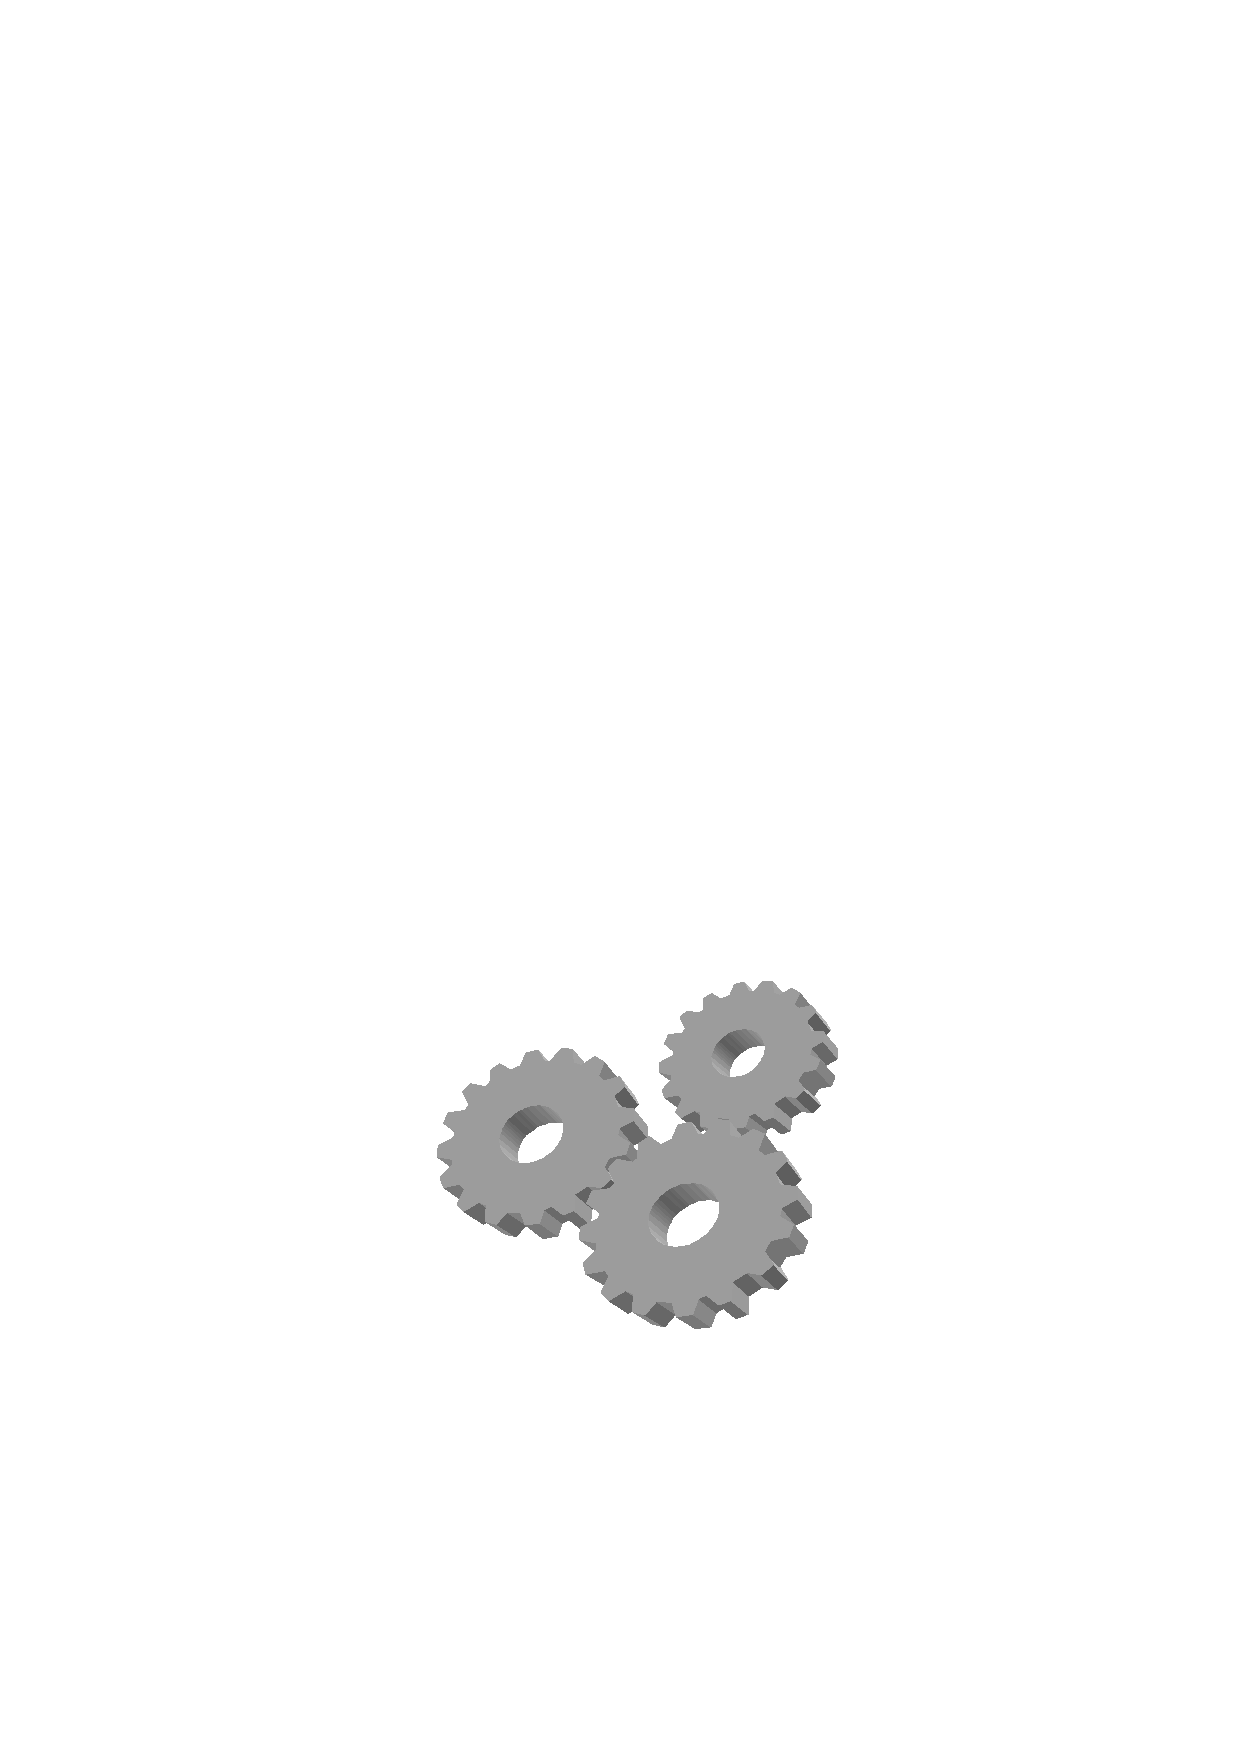
\includegraphics{picmain}
\caption{图 1.1 名称}
\end{figure}

\subsubsection{(1.1.1.1 题目)}
正文内容

正文内容

正文内容

\subsubsection{(1.1.1.2 题目)}
正文内容

正文内容

正文内容

\subsection{(1.1.2 题目)}
正文内容

正文内容

\begin{figure}[htp]
\centering
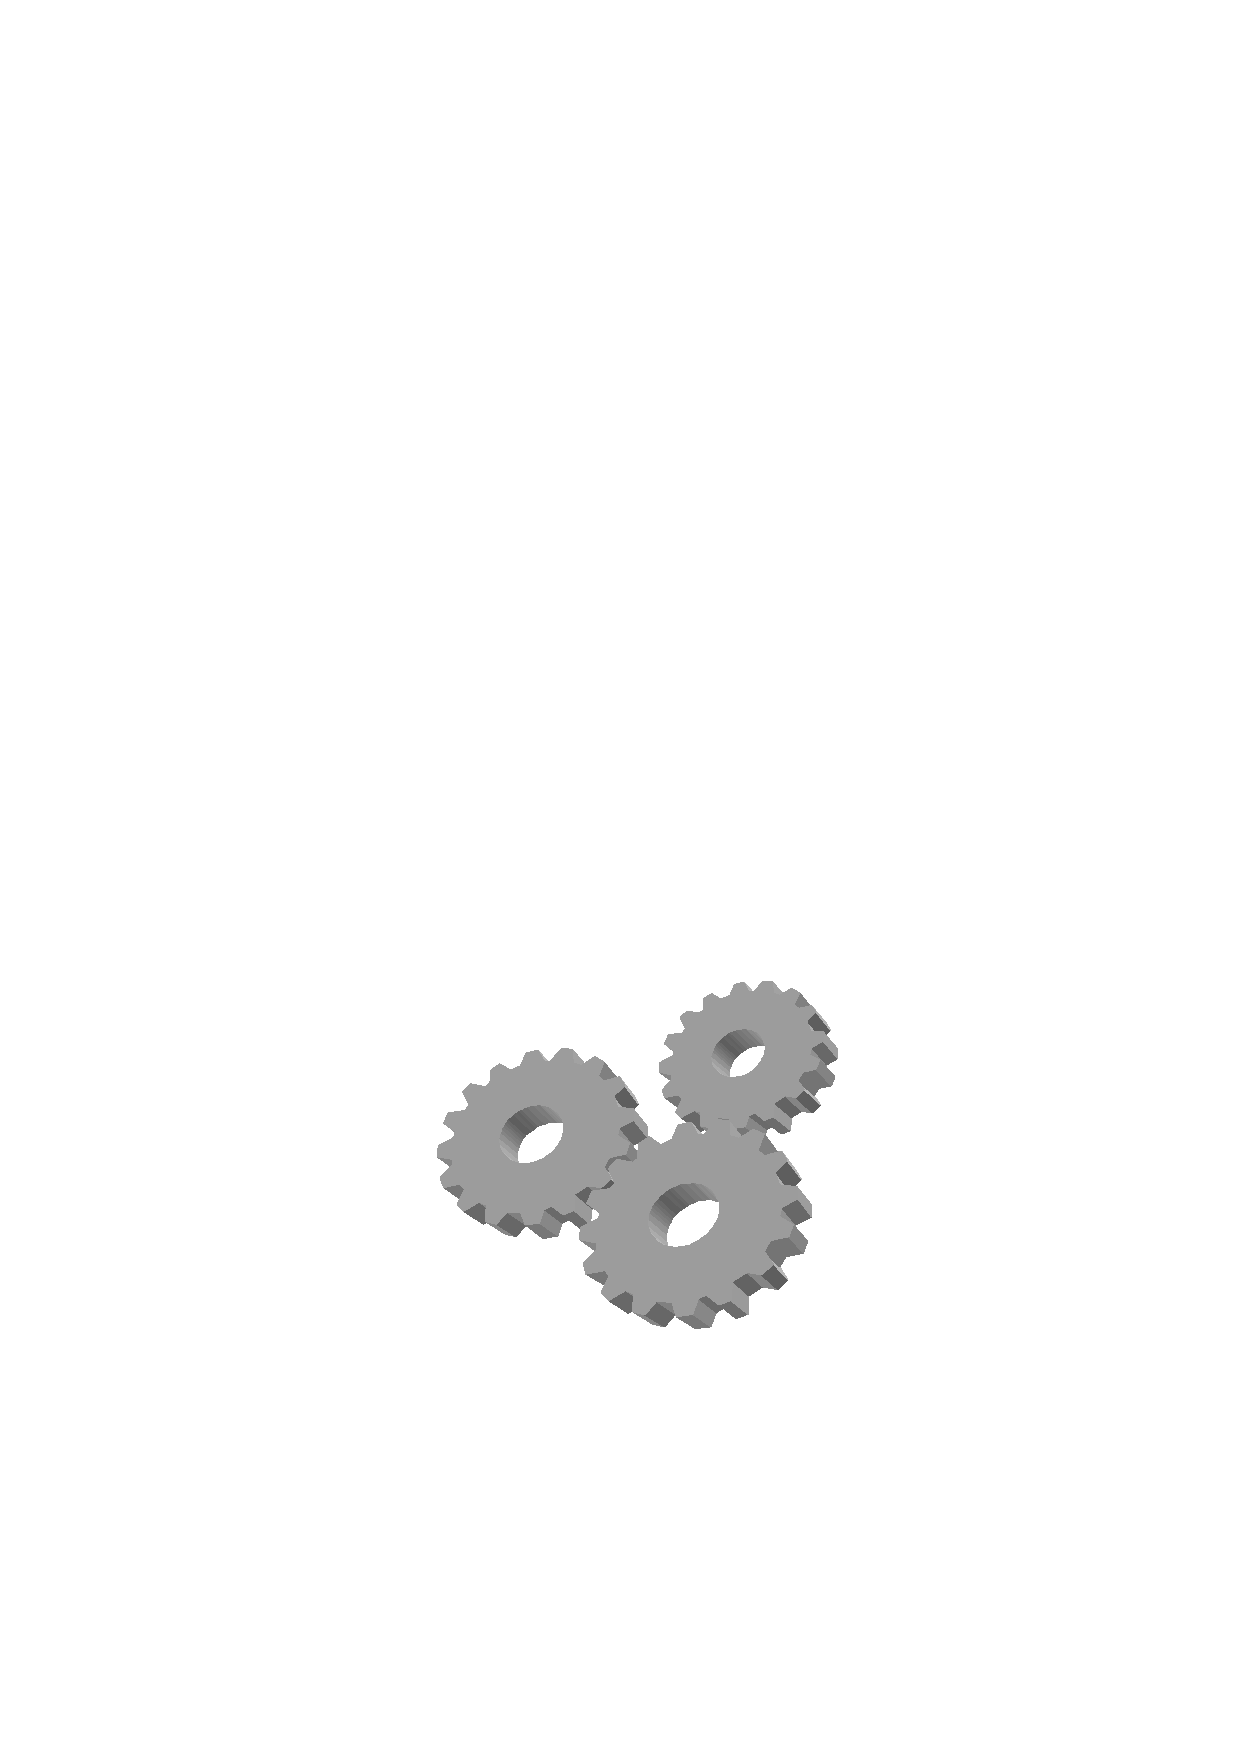
\includegraphics{picmain}
\caption{图 1.2 名称}
\end{figure}

\section{(1.2 题目)}
正文内容

正文内容

\begin{table}[htp]
\centering
\caption{表 1.2 名称}
\begin{tabular}{|c|c|c|c|c|}
\hline
\makebox[2.07cm][0pt]{} & \makebox[2.07cm][0pt]{} & \makebox[2.07cm][0pt]{} & \makebox[2.07cm][0pt]{} & \makebox[2.07cm][0pt]{} \\
\hline
 & & & & \\
\hline
 & & & & \\
\hline
\end{tabular}
\end{table}

正文内容

正文内容

正文内容

正文内容

\section{(1.3 题目)}
正文内容

正文内容

正文内容

正文内容

正文内容

正文内容

\subsection{(1.3.1 题目)}
正文内容

\begin{figure}[htp]
\centering
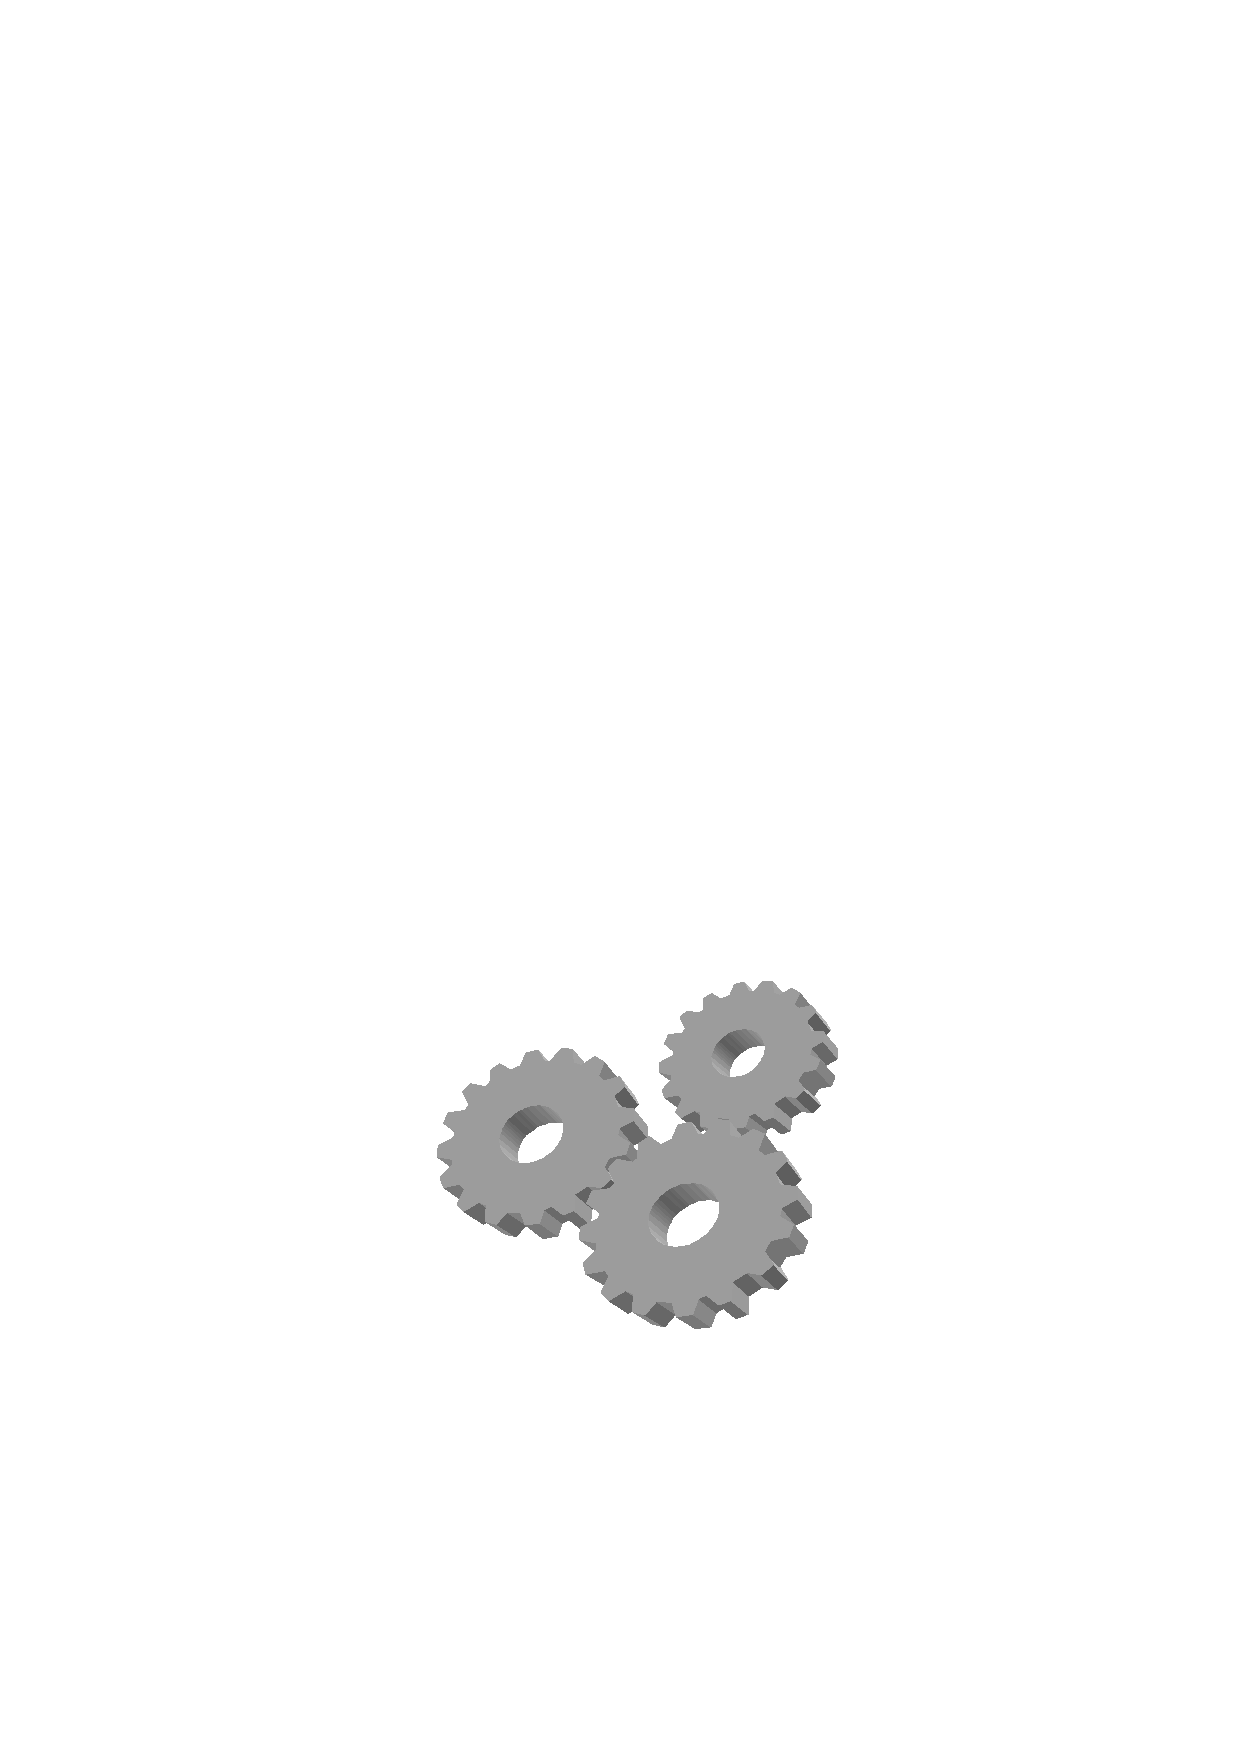
\includegraphics{picmain}
\caption{图 1.3 名称}
\end{figure}

\subsection{(1.3.2 题目)}
正文内容

正文内容

\begin{table}[htp]
\centering
\caption{表 1.2 名称}
\begin{tabular}{|c|c|c|c|c|}
\hline
\makebox[2.07cm][0pt]{} & \makebox[2.07cm][0pt]{} & \makebox[2.07cm][0pt]{} & \makebox[2.07cm][0pt]{} & \makebox[2.07cm][0pt]{} \\
\hline
 & & & & \\
\hline
 & & & & \\
\hline
\end{tabular}
\end{table}


\chapter{论文正文}
\label{chap:main}
本章将进入论文排版的正文, 按元素分主要包括:
{\kai 字体段落,图片表格,公式定理,参考文献}这几部分。
这个样例文件将包括模板中使用到的所有格式、模板中自定义命令到或者特有的东西,
都将被一一介绍,希望大家在排版自己的学位论文前能细致的看一遍,记住样例的格式和
方法,方便上手。

\section{字体段落}
\label{sec:font}

陈赓(1903年2月27日-1961年3月16日),原名陈庶康,中国湖南湘乡人,军事家。出生将门,其祖父为湘军将领陈翼怀。

Adobe中文字体有四种:

{\kai 楷体\verb|\kai|:陈赓,中国湖南湘乡人,军事家。出生将门,其祖父为湘军将领陈翼怀。%
1952年筹办并任人民解放军军事工程学院第一任院长兼政委,培养国防科技人才。1955年被授予大将军衔。}

{\fs 仿宋\verb|\fs|:陈赓,中国湖南湘乡人,军事家。出生将门,其祖父为湘军将领陈翼怀。%
1952年筹办并任人民解放军军事工程学院第一任院长兼政委,培养国防科技人才。1955年被授予大将军衔。}

{\hei 黑体\verb|\hei|:陈赓,中国湖南湘乡人,军事家。出生将门,其祖父为湘军将领陈翼怀。%
1952年筹办并任人民解放军军事工程学院第一任院长兼政委,培养国防科技人才。1955年被授予大将军衔。}

宋体就是正文字体了。下面测试字体大小,\LaTeX{}默认的列表环境会在
条目之间插入过多的行距,在下面这种情况可能正好,若用户需要
{\kai 正文行距}的列表环境,可以使用compactitem环境,记住这点很重要,不要再
用那种自己修改\verb|itemsep|的傻傻的办法了。
\begin{compactitem}
\item[初号] {\song\chuhao 陈赓大将}
\item[小初] {\song\xiaochu 陈赓大将}
\item[一号] {\song\yihao 陈赓大将}
\item[小一] {\song\xiaoyi 陈赓大将}
\item[二号] {\song\erhao 陈赓大将}
\item[小二] {\song\xiaoer 陈赓大将}
\item[三号] {\song\sanhao 陈赓大将}
\item[小三] {\song\xiaosan 陈赓大将}
\item[四号] {\song\sihao 陈赓大将}
\item[小四] {\song\xiaosi 陈赓大将}
\item[五号] {\song\wuhao 陈赓大将}
\item[小五] {\song\xiaowu 陈赓大将}
\end{compactitem}

\section{表格明细}
\label{sec:figure}
表格是论文的重要组成部分,我们从简单的表格讲起,到复杂的表格为止。

模板中关于表格的宏包有三个: \textsf{booktabs}、\textsf{array} 和
\textsf{longtabular}。三线表建议使用\textsf{booktabs}中提供的,
包含toprule、midrule 和 bottomrule三条命令,简单干脆!
它们与\textsf{longtable} 能很好的配合使用。下面来看一个表格实例:
\begin{table}[htb]
  \centering
  \begin{minipage}[t]{0.8\linewidth} % 如果想在表格中使用脚注,minipage是个不错的办法
  \caption[模板文件]{模板文件。如果表格的标题很长,那么在表格索引中就会很不美
    观,所以要像 chapter 那样在前面用中括号写一个简短的标题。这个标题会出现在索
    引中。}
  \label{tab:template-files}
    \begin{tabular*}{\linewidth}{lp{10cm}}
      \toprule[1.5pt]
      {\hei 文件名} & {\hei 描述} \\
      \midrule[1pt]
      nudtpaper.ins & \LaTeX{} 安装文件,docstrip\footnote{表格中的脚注} \\
      nudtpaper.dtx & 所有的一切都在这里面\footnote{再来一个}。\\
      nudtpaper.cls & 模板类文件。\\
      nudtpaper.cfg & 模板配置文。cls 和 cfg 由前两个文件生成。\\
      bstutf8.bst   & 参考文献 Bibtex 样式文件。\\
      mynudt.sty    & 常用的包和命令写在这里,减轻主文件的负担。\\
      \bottomrule[1.5pt]
    \end{tabular*}
  \end{minipage}
\end{table}

表 \ref{tab:template-files} 列举了本模板主要文件及其功能,基本上来说论文
中最可能用到的就是这种表格形式了。
请大家注意三线表中各条线对应的命令。这个例子还展示了如何在表格中正确使用脚注。
如果你不需要在表格中插入脚注,可以将minipage环境去掉。
由于\LaTeX{}本身不支持在表格中使用\verb|\footnote|,所以我们不得不将表格放在
小页中,而且最好将表格的宽度设置为小页的宽度,这样脚注看起来才更美观。

另外六院的同学在使用模板时需要使用一种固定宽度(往往是页宽,下面的例子由
rongdonghu提供)的表格,内容需要居中且可以自动调整。
解决办法是自定义了一种\verb|tabularx|中的\textbf{Z}环境,在论文模板中,
该命令已添加到\verb|mynudt.sty|中。下面是这种情况的实例:

\begin{table}[htbp]
\centering
\begin{minipage}[t]{0.9\linewidth}
\caption{Reed Solomon码的典型应用}
\label{tab:RSuse}
\begin{tabularx}{\linewidth}{cZ}
\toprule[1.5pt]
{\hei 应用领域} & {\hei 编码方案}\\
\midrule[1pt]
磁盘驱动器 & RS(32,28,5)码 \footnote{码长为32、维数为28、最小距离为5} \\
CD & 交叉交织RS码(CIRC) \\
DVD & RS(208,192,17)码、RS(182,172,11)码 \\
光纤通信 & RS(255,229,17)码 \\
\bottomrule[1.5pt]
\end{tabularx}
\end{minipage}
\end{table}

我们经常会在表格下方标注数据来源,或者对表格里面的条目进行解释。前面的脚注是一种
不错的方法,如果你不喜欢minipage方法的脚注。
那么完全可以在表格后面自己写注释,比如表~\ref{tab:tabexamp1}。
\begin{table}[htbp]
  \centering
  \caption{复杂表格示例 1}
  \label{tab:tabexamp1}
  \begin{minipage}[t]{0.8\textwidth}
    \begin{tabularx}{\linewidth}{|l|X|X|X|X|}
      \hline
      \multirow{2}*{\backslashbox{x}{y}}  & \multicolumn{2}{c|}{First Half} & \multicolumn{2}{c|}{Second Half}\\
      \cline{2-5}
      & 1st Qtr &2nd Qtr&3rd Qtr&4th Qtr \\
      \hline
      \multirow{2}*{East$^{*}$} &   20.4&   27.4&   90&     20.4 \\
       &   30.6 &   38.6 &   34.6 &  31.6 \\
      West$^{**}$ &   30.6 &   38.6 &   34.6 &  31.6 \\
      \hline
    \end{tabularx}\\[2pt]
    \footnotesize
    *:东部\\
    **:西部
  \end{minipage}
\end{table}

此外,表~\ref{tab:tabexamp1} 同时还演示了另外三个功能:1)通过 \textsf{tabularx} 的
 \texttt{|X|} 扩展实现表格内容自动调整;2)通过命令 \verb|\backslashbox| 在表头部分
插入反斜线(WORD中很简单,但\LaTeX{}做表格需要一定的(极大的)想象力);3)就是
使用\verb|multirow|和\verb|multicolumn|命令。

不可否认 \LaTeX{} 的表格功能没有想象中的那么强大,不过只要你足够认真,足够细致,那么
同样可以排出来非常复杂非常漂亮的表格。可是科技论文中那么复杂表格有什么用呢?
上面那个表格就够用啦。

浮动体的并排放置一般有两种情况:1)二者没有关系,为两个独立的浮动体;2)二者隶属
于同一个浮动体。对表格来说并排表格既可以像表~\ref{tab:parallel1}、表~\ref{tab:parallel2}
使用小页环境,也可以如表~\ref{tab:subtable}使用子表格来做。
图与表同出一源,后面我们将讲解子图(subfloat)的例子。
\begin{table}[htb]
\centering
\noindent\begin{minipage}{0.45\textwidth}
\centering
\caption{第一个并排子表格}
\label{tab:parallel1}
\begin{tabular}{p{2cm}p{2cm}}
\toprule[1.5pt]
111 & 222 \\\midrule[1pt]
222 & 333 \\\bottomrule[1.5pt]
\end{tabular}
\end{minipage}
\begin{minipage}{0.45\textwidth}
\centering
\caption{第二个并排子表格}
\label{tab:parallel2}
\begin{tabular}{p{2cm}p{2cm}}
\toprule[1.5pt]
111 & 222 \\\midrule[1pt]
222 & 333 \\\bottomrule[1.5pt]
\end{tabular}
\end{minipage}
\end{table}
\begin{table}[htbp]
\centering
\caption{并排子表格}
\label{tab:subtable}
\subfloat[第一个子表格]{
\begin{tabular}{p{2cm}p{2cm}}
\toprule[1.5pt]
111 & 222 \\\midrule[1pt]
222 & 333 \\\bottomrule[1.5pt]
\end{tabular}}\hskip2cm
\subfloat[第二个子表格]{
\begin{tabular}{p{2cm}p{2cm}}
\toprule[1.5pt]
111 & 222 \\\midrule[1pt]
222 & 333 \\\bottomrule[1.5pt]
\end{tabular}}
\end{table}

如果您要排版的表格长度超过一页,那么推荐使用\textsf{longtable}命令。
这里随便敲入一些无关的文字,使得正文看上去不是那么的少。
表~\ref{tab:performance} 就是 \textsf{longtable} 的简单示例。
\begin{longtable}[c]{c*{6}{r}}
\caption{实验数据}\label{tab:performance}\\
\toprule[1.5pt]
 测试程序 & \multicolumn{1}{c}{正常运行} & \multicolumn{1}{c}{同步}
& \multicolumn{1}{c}{检查点}   & \multicolumn{1}{c}{卷回恢复}
& \multicolumn{1}{c}{进程迁移} & \multicolumn{1}{c}{检查点} 	\\
& \multicolumn{1}{c}{时间 (s)} & \multicolumn{1}{c}{时间 (s)}
& \multicolumn{1}{c}{时间 (s)} & \multicolumn{1}{c}{时间 (s)}
& \multicolumn{1}{c}{时间 (s)} &  文件(KB)			\\
\midrule[1pt]%
\endfirsthead%

\multicolumn{7}{c}{续表~\thetable\hskip1em 实验数据}\\

\toprule[1.5pt]
 测试程序 & \multicolumn{1}{c}{正常运行} & \multicolumn{1}{c}{同步}
& \multicolumn{1}{c}{检查点}   & \multicolumn{1}{c}{卷回恢复}
& \multicolumn{1}{c}{进程迁移} & \multicolumn{1}{c}{检查点} 	\\
& \multicolumn{1}{c}{时间 (s)} & \multicolumn{1}{c}{时间 (s)}
& \multicolumn{1}{c}{时间 (s)} & \multicolumn{1}{c}{时间 (s)}
& \multicolumn{1}{c}{时间 (s)} &  文件(KB)			\\
\midrule[1pt]%
\endhead%
\hline%

\multicolumn{7}{r}{续下页}%

\endfoot%
\endlastfoot%
CG.A.2 & 23.05   & 0.002 & 0.116 & 0.035 & 0.589 & 32491  \\
CG.A.4 & 15.06   & 0.003 & 0.067 & 0.021 & 0.351 & 18211  \\
CG.A.8 & 13.38   & 0.004 & 0.072 & 0.023 & 0.210 & 9890   \\
CG.B.2 & 867.45  & 0.002 & 0.864 & 0.232 & 3.256 & 228562 \\
CG.B.4 & 501.61  & 0.003 & 0.438 & 0.136 & 2.075 & 123862 \\
CG.B.8 & 384.65  & 0.004 & 0.457 & 0.108 & 1.235 & 63777  \\
MG.A.2 & 112.27  & 0.002 & 0.846 & 0.237 & 3.930 & 236473 \\
MG.A.4 & 59.84   & 0.003 & 0.442 & 0.128 & 2.070 & 123875 \\
MG.A.8 & 31.38   & 0.003 & 0.476 & 0.114 & 1.041 & 60627  \\
MG.B.2 & 526.28  & 0.002 & 0.821 & 0.238 & 4.176 & 236635 \\
MG.B.4 & 280.11  & 0.003 & 0.432 & 0.130 & 1.706 & 123793 \\
MG.B.8 & 148.29  & 0.003 & 0.442 & 0.116 & 0.893 & 60600  \\
LU.A.2 & 2116.54 & 0.002 & 0.110 & 0.030 & 0.532 & 28754  \\
LU.A.4 & 1102.50 & 0.002 & 0.069 & 0.017 & 0.255 & 14915  \\
LU.A.8 & 574.47  & 0.003 & 0.067 & 0.016 & 0.192 & 8655   \\
LU.B.2 & 9712.87 & 0.002 & 0.357 & 0.104 & 1.734 & 101975 \\
LU.B.4 & 4757.80 & 0.003 & 0.190 & 0.056 & 0.808 & 53522  \\
LU.B.8 & 2444.05 & 0.004 & 0.222 & 0.057 & 0.548 & 30134  \\
EP.A.2 & 123.81  & 0.002 & 0.010 & 0.003 & 0.074 & 1834   \\
EP.A.4 & 61.92   & 0.003 & 0.011 & 0.004 & 0.073 & 1743   \\
EP.A.8 & 31.06   & 0.004 & 0.017 & 0.005 & 0.073 & 1661   \\
EP.B.2 & 495.49  & 0.001 & 0.009 & 0.003 & 0.196 & 2011   \\
EP.B.4 & 247.69  & 0.002 & 0.012 & 0.004 & 0.122 & 1663   \\
EP.B.8 & 126.74  & 0.003 & 0.017 & 0.005 & 0.083 & 1656   \\
\bottomrule[1.5pt]
\end{longtable}

另外,有的同学不想让某个表格或者图片出现在索引里面,那么请使用命令 \verb|\caption*{}|,
这个命令不会给表格编号,也就是出来的只有标题文字而没有“表~XX”,“图~XX”,否则
索引里面序号{\kai 不连续}就显得不伦不类,这也是 \LaTeX{} 里星号命令默认的规则。

\section{绘图插图}

本模板不再预先装载任何绘图包(如 \textsf{pstricks,pgf} 等),完全由你自己来决定。
个人觉得 \textsf{pgf} 不错,不依赖于 Postscript。此外还有很多针对 \LaTeX{} 的
 GUI 作图工具,如 XFig(jFig), WinFig, Tpx, Ipe, Dia, Inkscape, LaTeXPiX,
jPicEdt 等等。本人强烈推荐\textsf{Ipe}。

一般图形都是处在浮动环境中。之所以称为浮动是指最终排版效果图形的位置不一定与源文
件中的位置对应,这也是刚使用 \LaTeX{} 同学可能遇到的问题。
如果要强制固定浮动图形的位置,请使用 \textsf{float} 宏包,
它提供了 \texttt{[H]}(意思是图片就给我放在这里\textcolor{red}{H}ere)参数,
但是除非特别需要,不建议使用\texttt{[H]},而是推荐使用\texttt{[htbp]},
给\LaTeX{}更多选择。比如图~\ref{fig:ipe}。
\begin{figure}[htbp] % use float package if you want it here
  \centering
  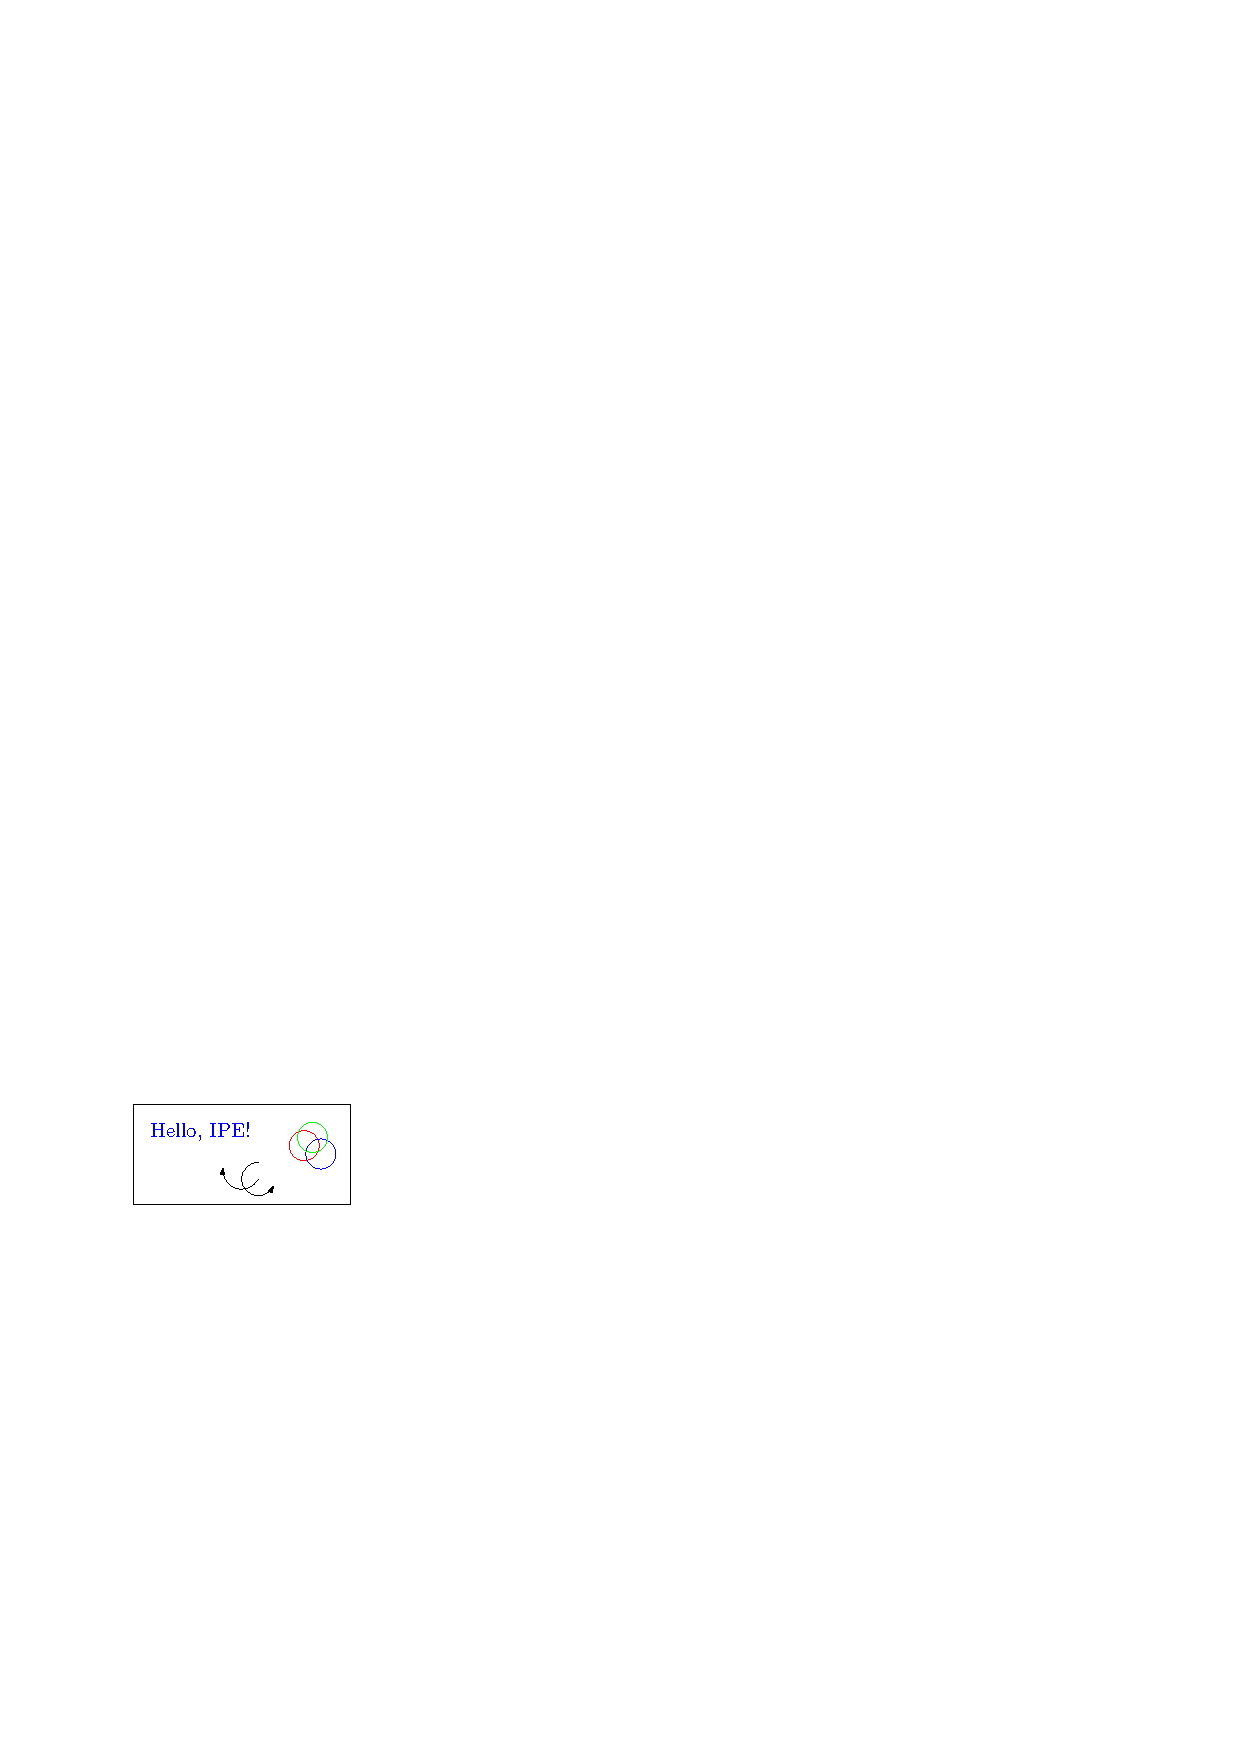
\includegraphics[width=3in]{hello}
  \caption{利用IPE制图}
  \label{fig:ipe}
\end{figure}

若子图共用一个计数器,
那么请看图~\ref{fig:big1},它包含两个小图,分别是图~\ref{fig:subfig1}
和图~\ref{fig:subfig2}。这里推荐使用\verb|\subfloat|,{\bf 不要再用}
\verb|\subfigure|和\verb|\subtable|。
\begin{figure}[htb]
  \centering%
  \subfloat[第一个小图形]{%
    \label{fig:subfig1}
    
\includegraphics[height=2cm]{xh}}\hspace{4em}%
  \subfloat[第二个小图形。如果标题很长的话,它会自动换行,这个 caption 就是这样的例子]{%
    \label{fig:subfig2}
    
\includegraphics[height=2cm]{xhh}}
  \caption{包含子图形的大图形}
  \label{fig:big1}
\end{figure}

而下面这个例子显示并排$3\times2$的图片,见图\ref{fig:subfig:3x2}:
\begin{figure}[htb]
\centering
\subfloat[]{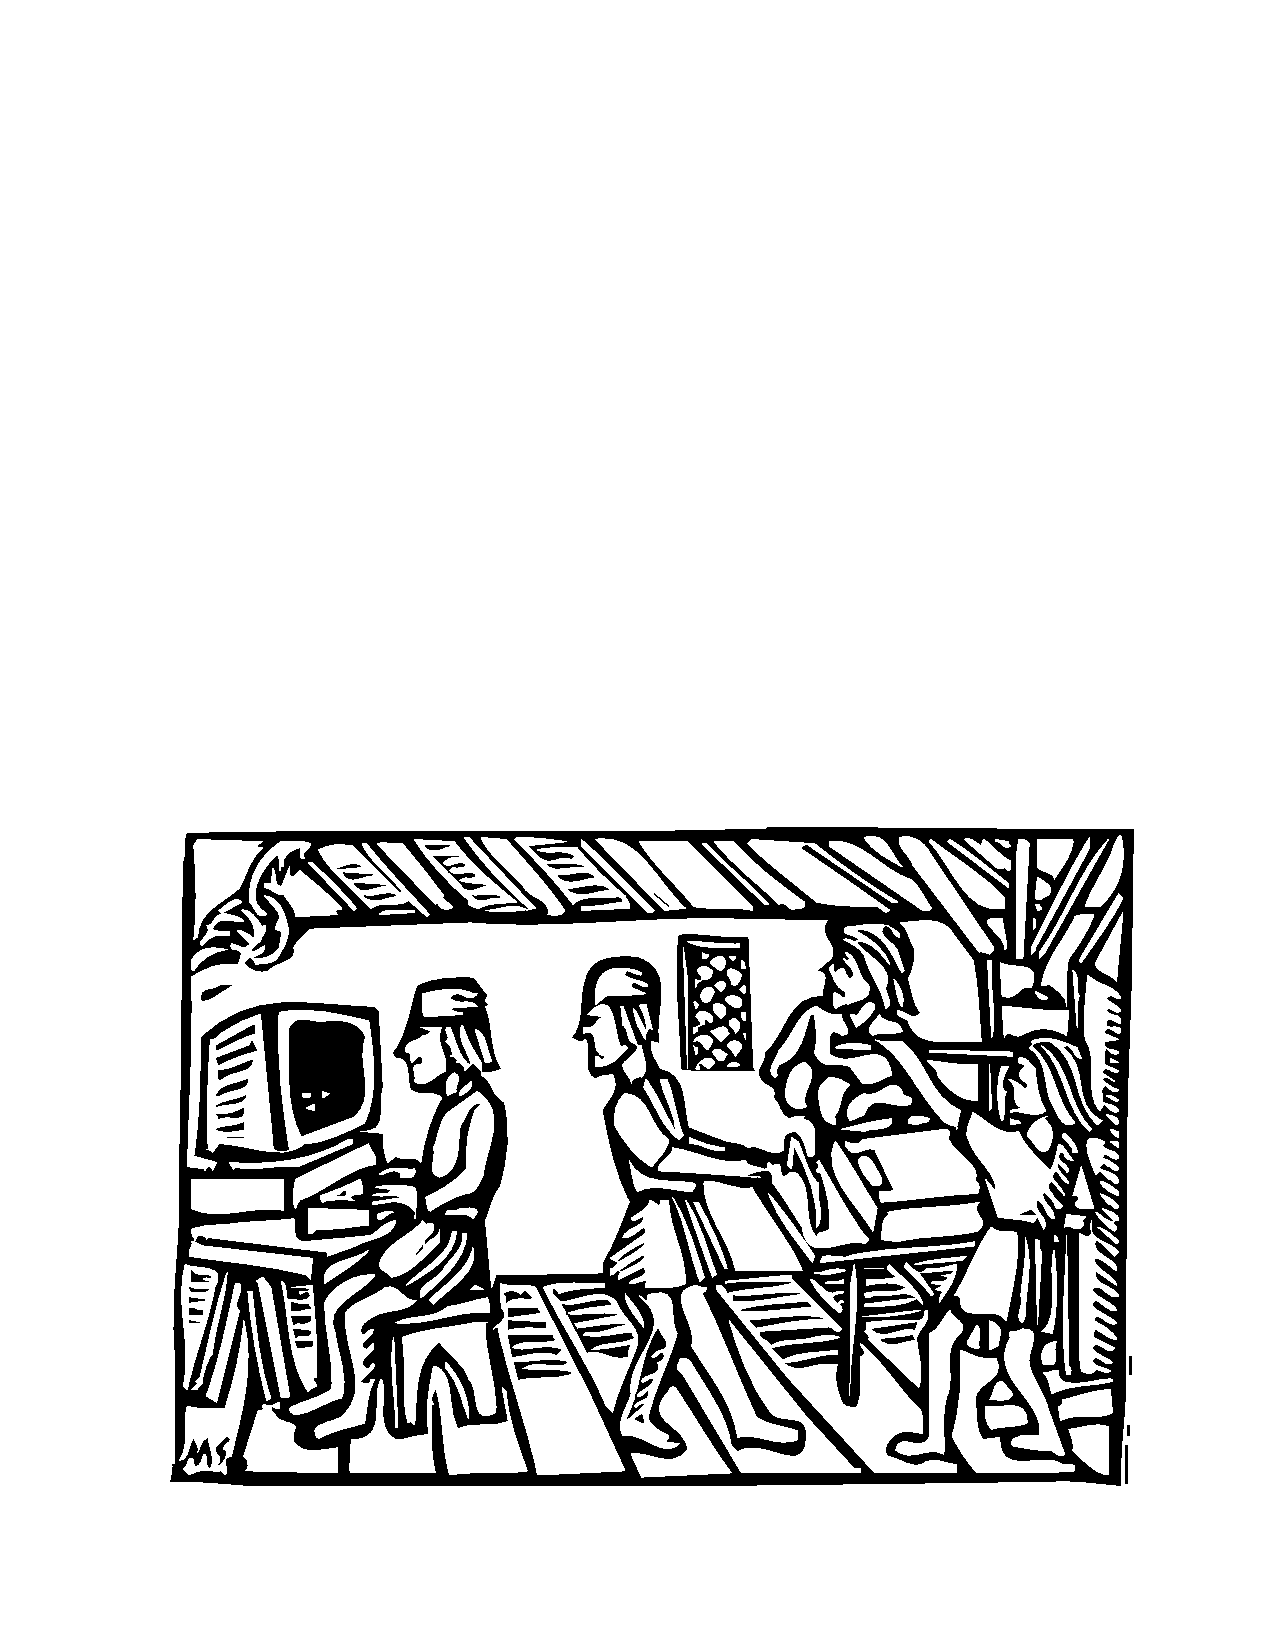
\includegraphics[width=.27\textwidth]{typography}} \qquad
\subfloat[]{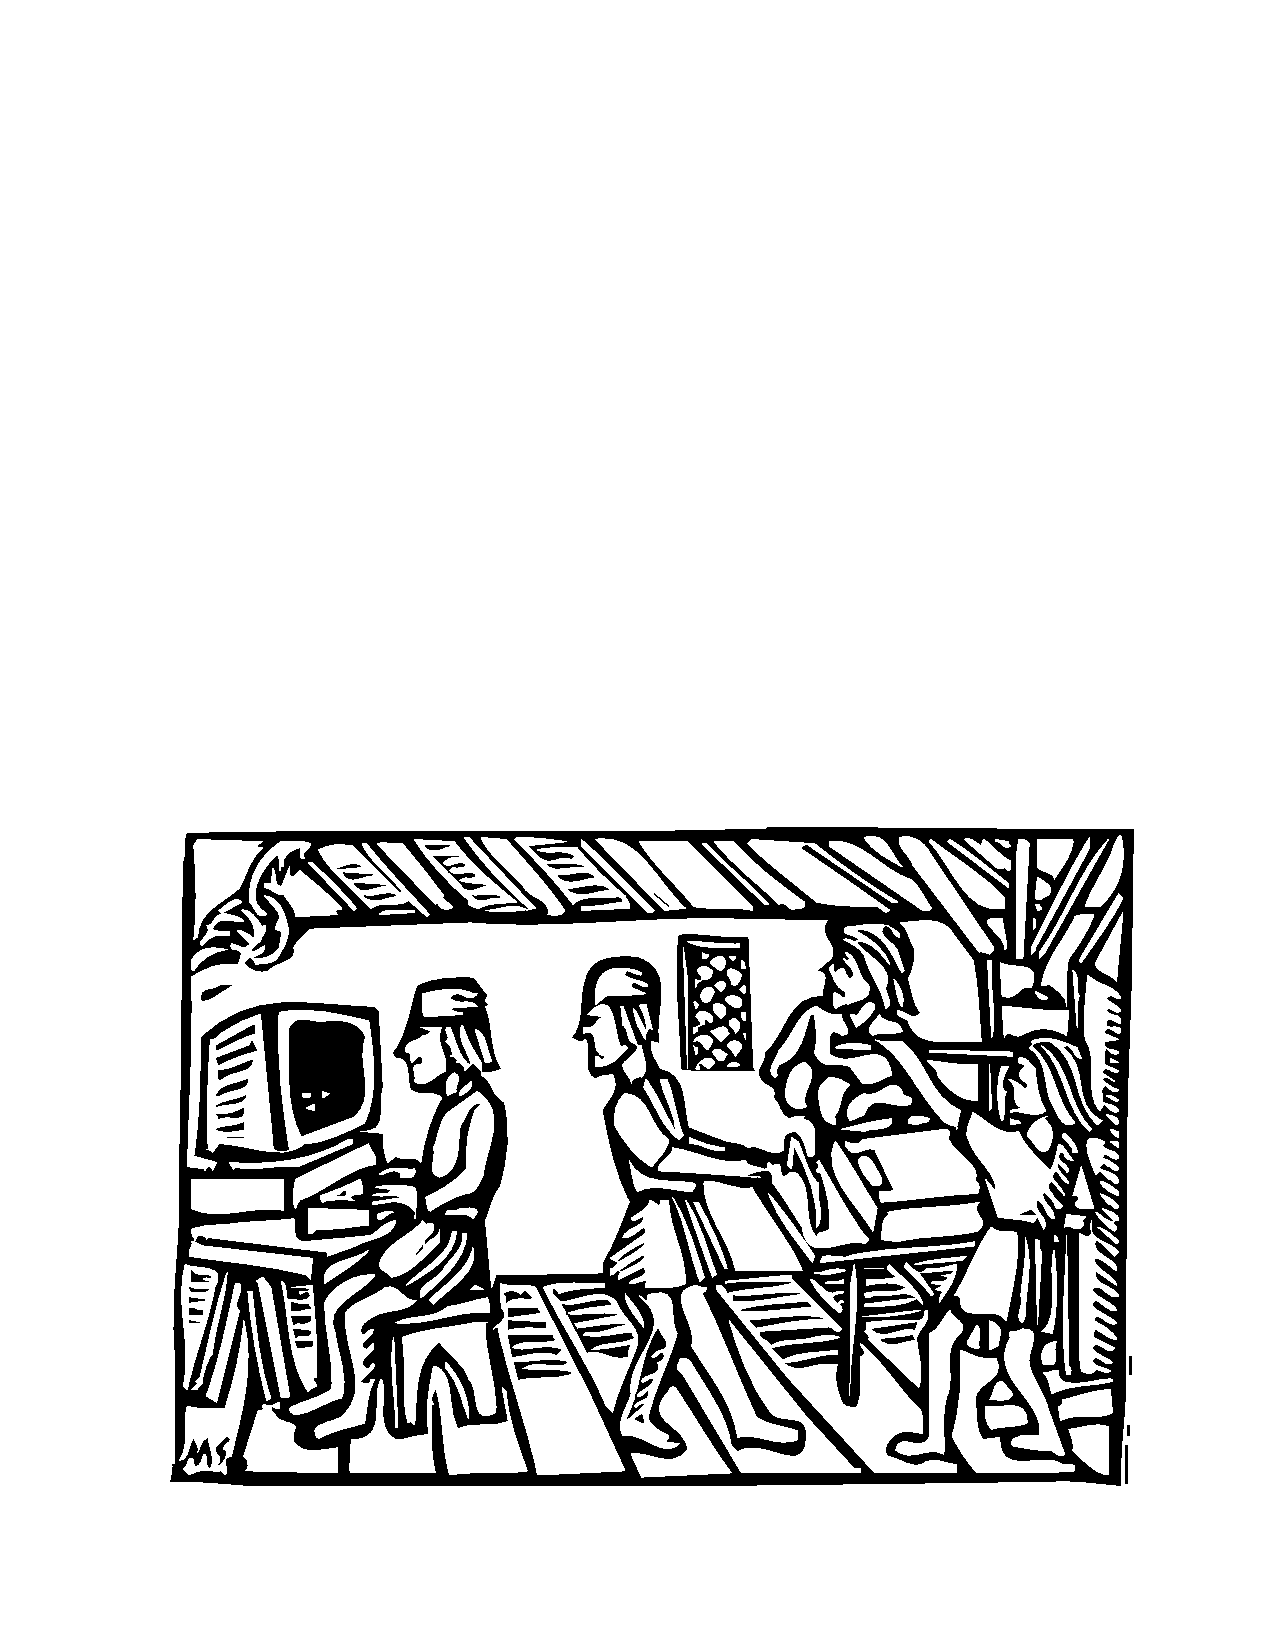
\includegraphics[width=.27\textwidth]{typography}} \qquad
\subfloat[]{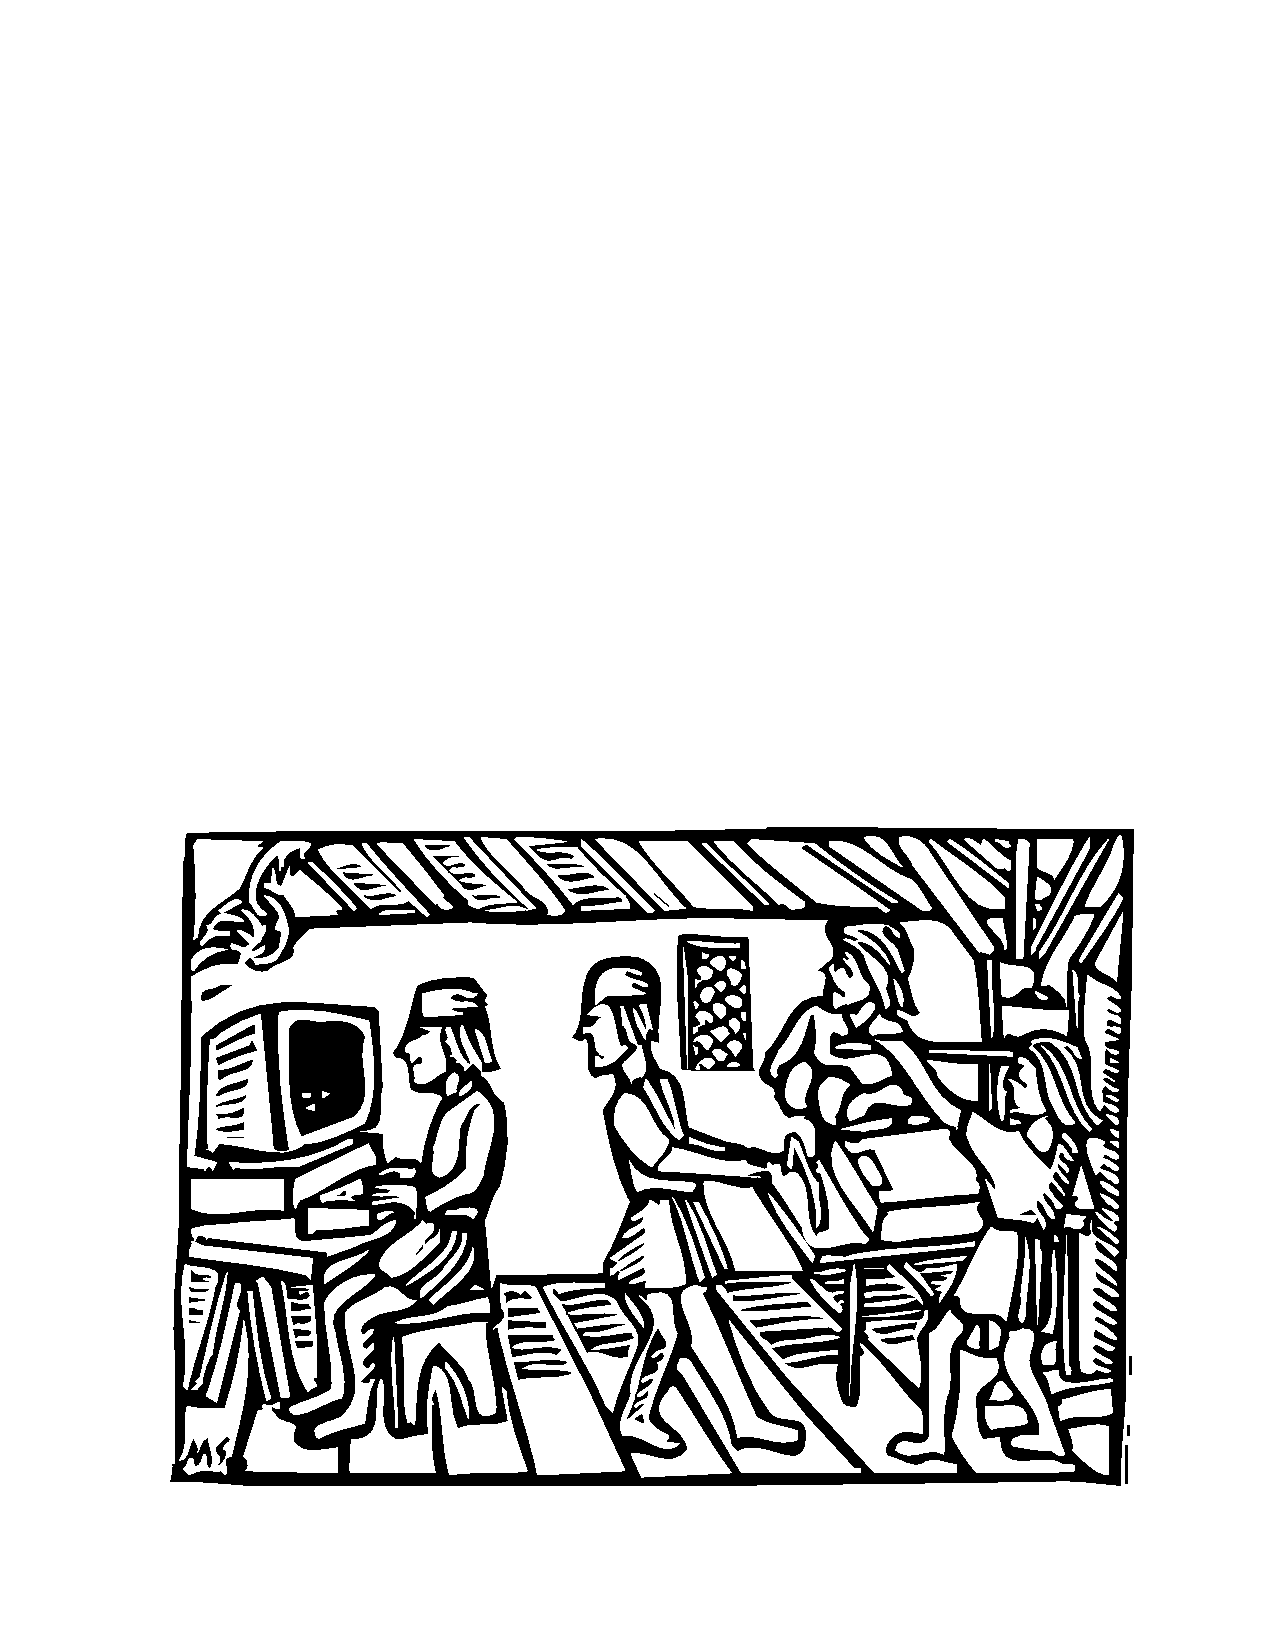
\includegraphics[width=.27\textwidth]{typography}} \qquad
\subfloat[]{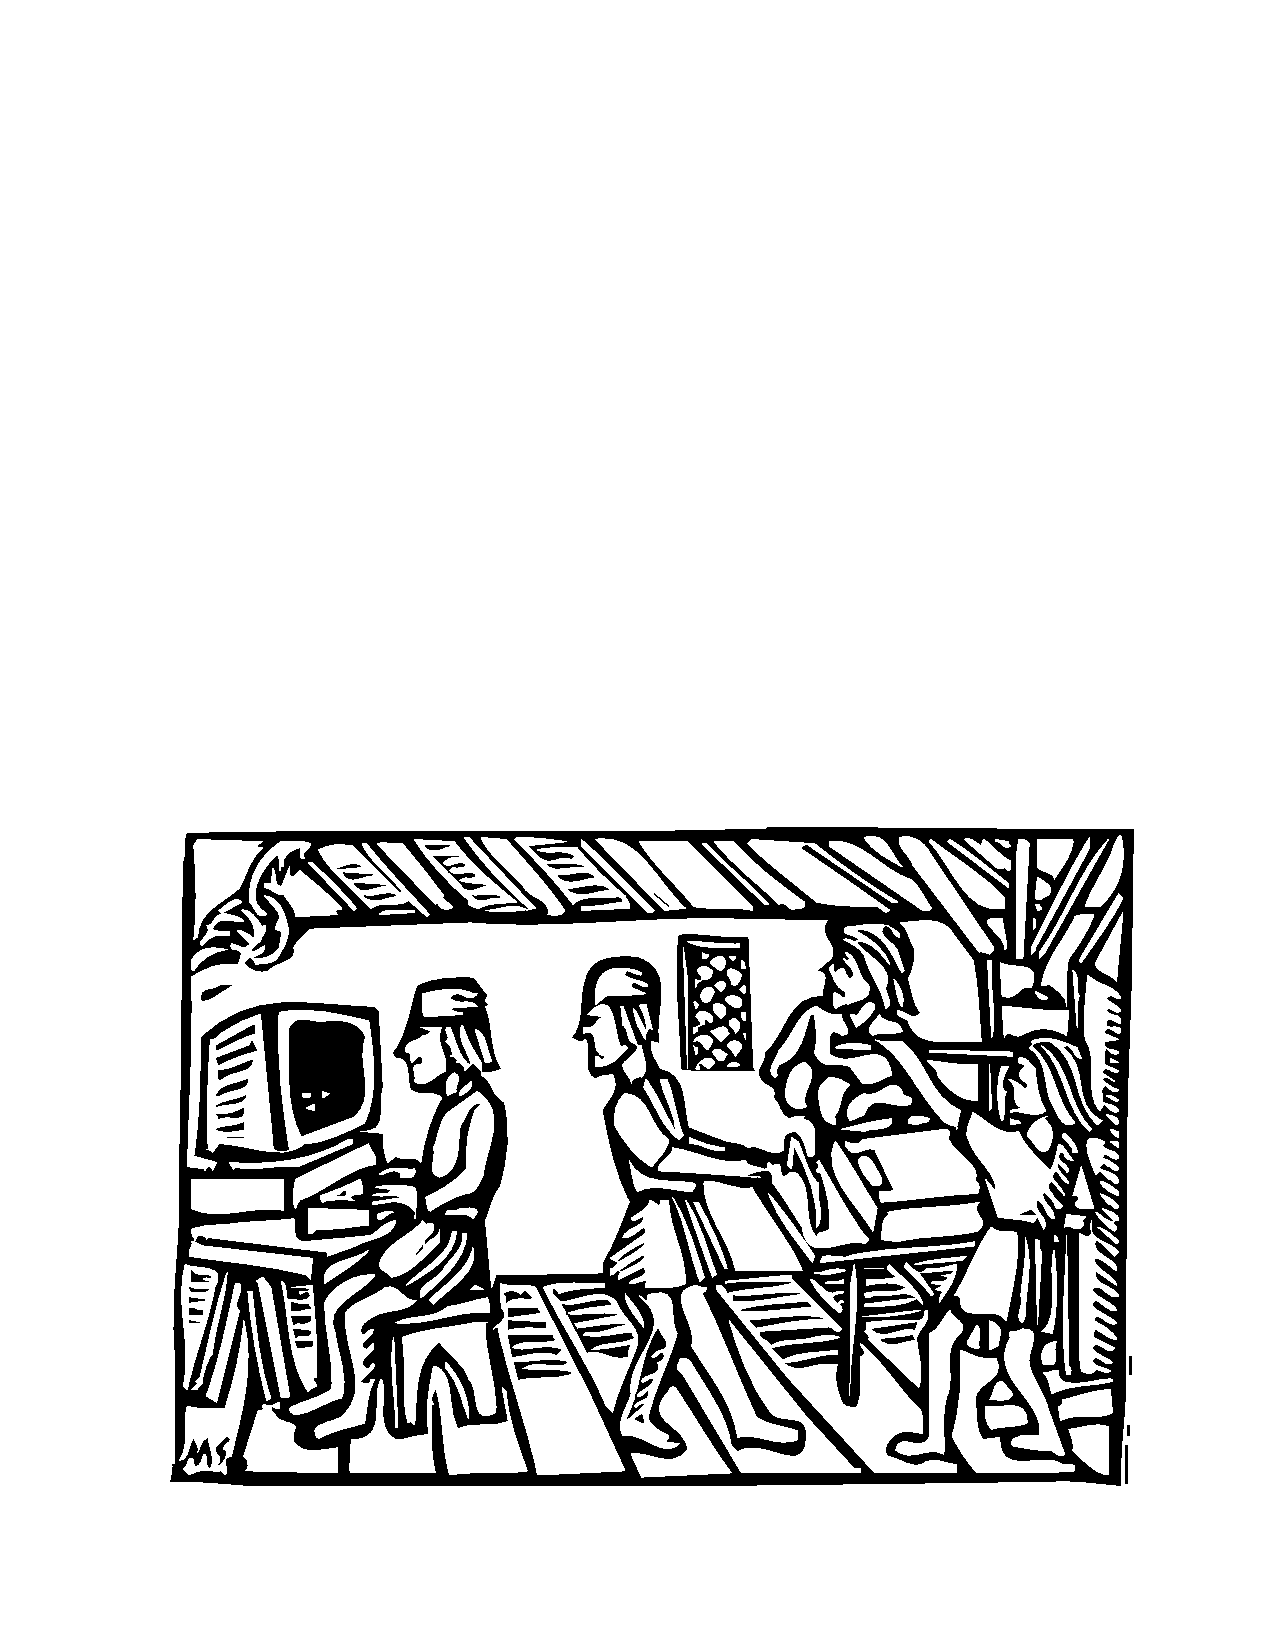
\includegraphics[width=.27\textwidth]{typography}} \qquad
\subfloat[]{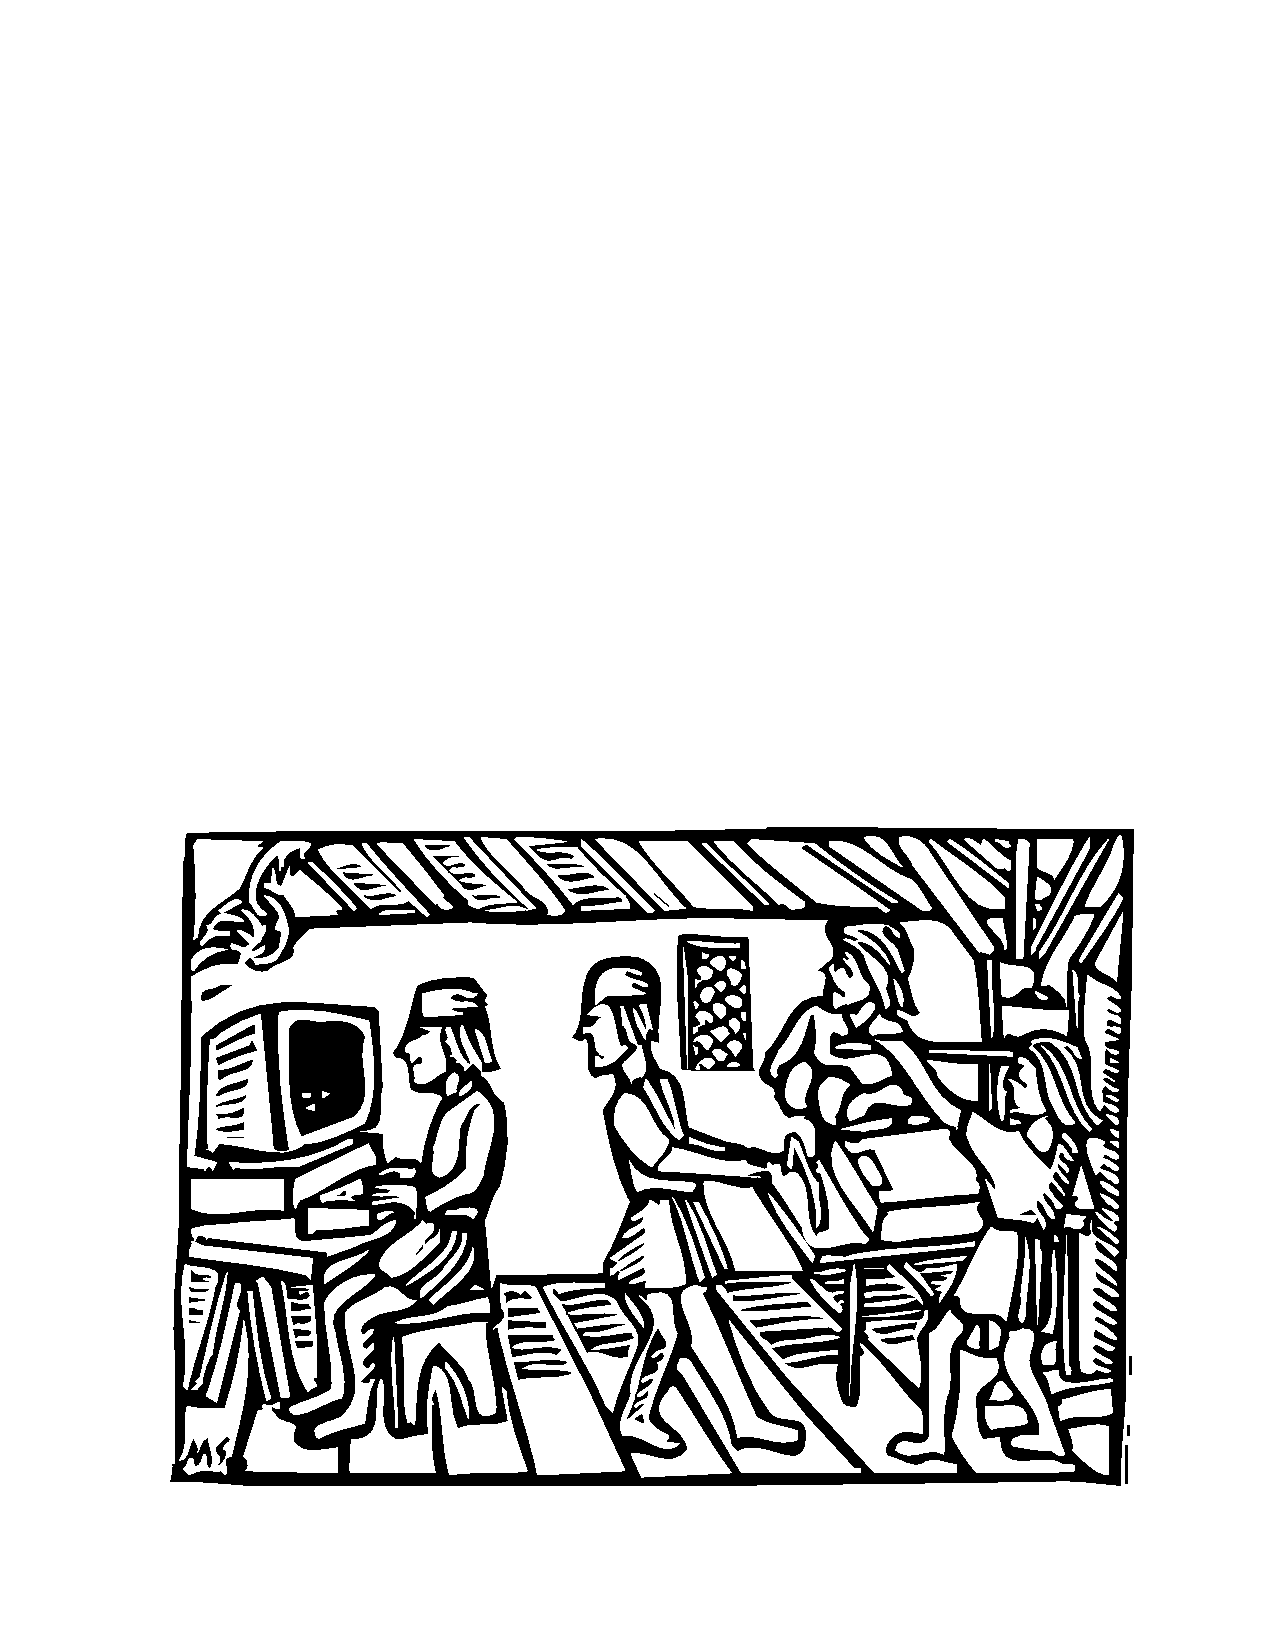
\includegraphics[width=.27\textwidth]{typography}} \qquad
\subfloat[]{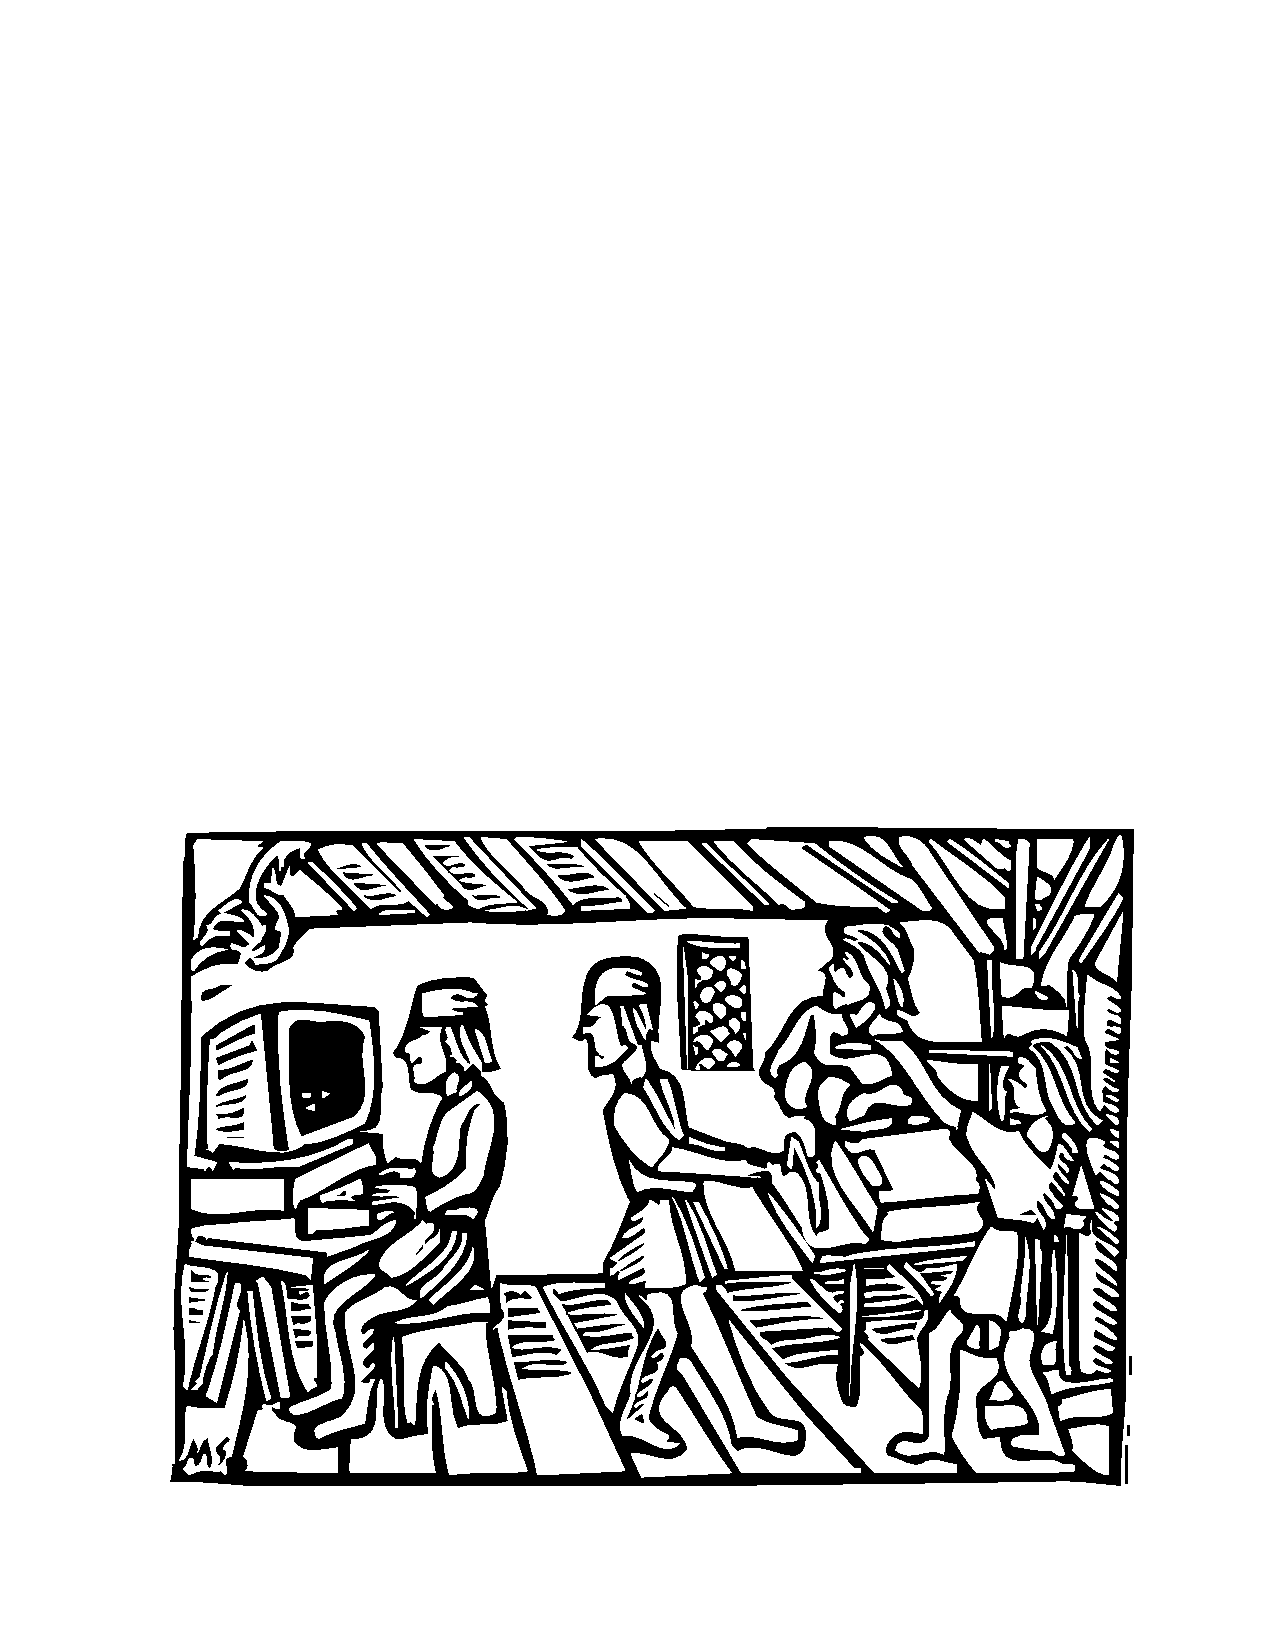
\includegraphics[width=.27\textwidth]{typography}}
\caption{并排图片}
\label{fig:subfig:3x2}
\end{figure}

要注意,图\ref{fig:subfig:3x2}例中
\texttt{qquad}相当于\verb|\hspace{2em}|,也就是2个字符的宽度,约0.08倍页宽,
图片宽度设定为0.27倍页宽是合适的;在该环境中,尽量不要手动换行,所以,不妨自己计算一下!

如果要把编号的两个图形并排,那么小页(minipage)就非常有用了,可以分别参考
图\ref{fig:parallel1}和图\ref{fig:parallel2}。其实这个例子和表格一节中并排
放置的表格一摸一样。
\begin{figure}[htb]
\begin{minipage}{0.48\textwidth}
  \centering
  
\includegraphics[height=1.2cm]{xhh}
  \caption{并排第一个图}
  \label{fig:parallel1}
\end{minipage}\hfill
\begin{minipage}{0.48\textwidth}
  \centering
  
\includegraphics[height=1.2cm]{xhh}
  \caption{并排第二个图}
  \label{fig:parallel2}
\end{minipage}
\end{figure}

图形就说这么多,因为大家在写论文是遇到的最大问题不是怎么把图插进去,
而是怎样做出专业的、诡异的、震撼的图片来,记得在这时参考前面推荐的那
些工具吧,当然必不可少的是Matlab了,至于如何加入中文标注、支持中文等等
可以上网去查,但这里{\kai 推荐一点},用好export命令,使得插入图片时尽可能的不要
缩放,保证图文的一致性。

\section{公式定理}
\label{sec:equation}
贝叶斯公式如式~(\ref{equ:chap1:bayes}),其中$p(y|\mathbf{x})$为后验;
$p(\mathbf{x})$为先验;分母$p(\mathbf{x})$ 为归一化因子,这是
实际应用中十分恐怖的一个积分式。
\begin{equation}
\label{equ:chap1:bayes}
p(y|\mathbf{x}) = \frac{p(\mathbf{x},y)}{p(\mathbf{x})}=
\frac{p(\mathbf{x}|y)p(y)}{p(\mathbf{x})}
\end{equation}

论文里面公式越多,\TeX{} 就越 happy。再看一个 \textsf{amsmath} 的例子:
\newcommand{\envert}[1]{\left\lvert#1\right\rvert}
\begin{equation}\label{detK2}
\det\mathbf{K}(t=1,t_1,\dots,t_n)=\sum_{I\in\mathbf{n}}(-1)^{\envert{I}}
\prod_{i\in I}t_i\prod_{j\in I}(D_j+\lambda_jt_j)\det\mathbf{A}
^{(\lambda)}(\overline{I}|\overline{I})=0.
\end{equation}

大家在写公式的时候一定要好好看\textsf{amsmath}的文档,并参考模板中的用法:
\begin{multline*}%\tag{[b]} % 这个出现在索引中的
\int_a^b\biggl\{\int_a^b[f(x)^2g(y)^2+f(y)^2g(x)^2]
 -2f(x)g(x)f(y)g(y)\,dx\biggr\}\,dy \\
 =\int_a^b\biggl\{g(y)^2\int_a^bf^2+f(y)^2
  \int_a^b g^2-2f(y)g(y)\int_a^b fg\biggr\}\,dy
\end{multline*}

再看\ref{equ:split}:
\begin{equation}\label{equ:split}
\begin{split}
C(z) &= [z^n] \biggl[\frac{e^{3/4}}{\sqrt{1-z}} +
e^{-3/4}(1-z)^{1/2} + \frac{e^{-3/4}}{4}(1-z)^{3/2}
+ O\Bigl( (1-z)^{5/2}\Bigr)\biggr] \\
&= \frac{e^{-3/4}}{\sqrt{\pi n}} - \frac{5e^{-3/4}}{8\sqrt{\pi
n^3}} + \frac{e^{-3/4}}{128 \sqrt{\pi n^5}} +
O\biggl(\frac{1}{\sqrt{\pi
n^7}}\biggr)
\end{split}
\end{equation}

当然了,数学中必不可少的是定理和证明:
\begin{theorem}
  \label{chapTSthm:rayleigh solution}
  假定 $X$ 的二阶矩存在:
  \begin{equation}
         O_R(\mathbf{x},F)=\sqrt{\frac{\mathbf{u}_1^T\mathbf{A}\mathbf{u}_1} {\mathbf{u}_1^T\mathbf{B}\mathbf{u}_1}}=\sqrt{\lambda_1},
  \end{equation}
  其中 $\mathbf{A}$ 等于 $(\mathbf{x}-EX)(\mathbf{x}-EX)^T$,$\mathbf{B}$ 表示协方差阵 $E(X-EX)(X-EX)^T$,$\lambda_1$
$\mathbf{u}_1$是$\lambda_1$对应的特征向量,
\end{theorem}

对于希腊符号使用\verb|mathbf|命令可能有些问题,所以建议对符号
用\verb|bm|加粗,记得用\verb|\up<greek>|切换正体符号,下面看几个例子:
\verb|\gamma|斜体代表变量$\gamma$,\verb|\bm{\upgamma}|正体代表向量$\bm{\upgamma}$,
。\verb|\Gamma|正体代表操作符号$\Gamma$,
\verb|\bm{\Gamma}|正体粗体代表矩阵形式$\bm{\Gamma}$,
\verb|\varGamma|斜体代表变量$\varGamma$。另外对于大小写斜体的加粗可以见$\bm{\gamma}$和$\bm{\varGamma}$,
但是这两种科技论文中很少出现,这里只做测试。
非符号普通向量就用\verb|\mathbf|吧:$\mathbf{x}_k,\mathbf{X}_k$。
完整测试如下$\omega,\bm{\omega},\upomega,\bm{\upomega},\Omega,\bm{\Omega},\varOmega,\bm{\varOmega}$。

\begin{proof}
上述优化问题显然是一个Rayleigh商问题。我们有
  \begin{align}
     O_R(\mathbf{x},F)=\sqrt{\frac{\mathbf{u}_1^T\mathbf{A}\mathbf{u}_1} {\mathbf{u}_1^T\mathbf{B}\mathbf{u}_1}}=\sqrt{\lambda_1},
 \end{align}
 其中 $\lambda_1$ 下列广义特征值问题的最大特征值:
$$
\mathbf{A}\mathbf{z}=\lambda\mathbf{B}\mathbf{z}, \mathbf{z}\neq 0.
$$
 $\mathbf{u}_1$ 是 $\lambda_1$对应的特征向量。结论成立。
\end{proof}

下面来看看算法环境的定义和使用。
我们知道,故障诊断的最终目的,是将故障定位到部件,而由于信号--部件依赖矩阵的存在,因此,实质性的工作是找出由故障部件发出异常信号,
不妨称为源异常信号,而如前所述,源异常信号与异常信号依赖矩阵$\mathbf{S_a}$的全零列是存在一一对应的关系的。因此,我们只要获得了$\mathbf{S_a}$的全零列的相关信息,
也就获得了源异常信号的信息,从而能进一步找到故障源。
通过以上分析,我们构造算法\ref{alg53},用于实现非回路故障诊断。
\begin{algorithm}[htbp]
  \caption{非回路故障诊断算法}
  \label{alg53}
  \begin{algorithmic}[1]
    \REQUIRE 信号--部件依赖矩阵$\mathbf{A}$,信号依赖矩阵$\mathbf{S}$,信号状态向量$\alpha$
    \ENSURE 部件状态向量$\gamma$
    \STATE $\mathbf{P}\leftarrow\left(<\alpha>\right)$
    \STATE $\mathbf{S_{a}}\leftarrow\mathbf{P^T}\mathbf{S}\mathbf{P}$
    \FOR{$i=1$ to $S_a$的阶数$m$}
    \STATE $s_i\leftarrow s_i$的第$i$个行向量
    \ENDFOR
    \STATE $\beta_a\leftarrow\lnot \left(s_1\lor s_2\lor \cdots\lor s_m\right)^T$
    \STATE $\beta\leftarrow\mathbf{P}\beta_a$
    \STATE $\gamma\leftarrow\mathbf{A}\beta$
  \end{algorithmic}
\end{algorithm}

第一类故障回路推理与非回路故障推理是算法基本相同,稍微不同的是$\beta_a$的计算。因为第一类故障回路中的信号全部可能是源异常信号,因此我们不必计算
$\beta_a=\lnot \left(\left[s_1\lor s_2\lor \cdots\lor s_m\right]^T\right)$,而直接取$\beta_a=\underbrace{\left[\begin{array}{cccc}1&1&\cdots&1\end{array}\right]^T}_m$,将$\beta_a$代入
算法\ref{alg53},有
\[\beta=\mathbf{P}\beta_a=\mathbf{P}\underbrace{\left[\begin{array}{cccc}1&1&\cdots&1\end{array}\right]^T}_m=\alpha\]
因此一类故障回路的推理算法变得相当简单,例如算法\ref{alg54}
\begin{algorithm}[htbp]
  \caption{第一类故障回路诊断算法}
  \label{alg54}
  \begin{algorithmic}[1]
    \REQUIRE 信号--部件依赖矩阵$\mathbf{A}$,信号状态向量$\alpha$
    \ENSURE 部件状态向量$\gamma$
    \STATE $\gamma\leftarrow\mathbf{A}\alpha$
  \end{algorithmic}
\end{algorithm}

\section{参考文献}
\label{sec:bib}
当然参考文献可以直接写 bibitem,虽然费点功夫,但是好控制,各种格式可以自己随意改
写,在nudtpaper里面,建议使用JabRef编辑和管理文献,再结合指定的样式,
对中文的支持非常不错,格式也很规范。

本模板推荐使用 biblatex,即使用biber编译文献数据,文献样式基于gb7714-2015样式针对科大要求专门定制。
上标标签的引用命令可使用\textcolor{blue}{\textbf{cite}}、upcite,
行内标签的引用命令可使用\textcolor{blue}{\textbf{parencite}}、inlinecite 等。例如:见文献
\cite{ref-1-1-周融,ref-2-2-夏鲁惠,ref-3-3-Heider,ref-4-3-刘国钧,ref-5-5-Gill},就是上标的例子。
见文献\parencite{ref-6-6-李大伦,ref-7-7-French,ref-8-8-伍蠡甫,ref-9-9-Spivak,ref-10-10-Almarza}就是行内非上标的例子。

本模板也可以使用 BIB\TeX,只要去掉文档类中biber选项即可,样式文件为 bstutf8.bst,符合学校的参考文献格式(如专利
等引用未加详细测试)。看看这个例子,关于书的\upcite{tex, companion},
还有这些\upcite{Krasnogor2004e, clzs, zjsw},关于杂志的\upcite{ELIDRISSI94,
  MELLINGER96, SHELL02},硕士论文\upcite{zhubajie, metamori2004},博士论文
\upcite{shaheshang, FistSystem01},标准文件\upcite{IEEE-1363},会议论文\upcite{DPMG,kocher99},%
技术报告\upcite{NPB2}。

使用bibtex时要特别注意:

中文参考文献\upcite{cnarticle},需要在bib文件对应文献条目中
增加\verb|language|域并设为\verb|zh|,英文此项可不填,之后由\verb|bstutf8|统一处理
(具体就是决定一些文献在中英文不同环境下的显示格式,如等、etc)。
若使用\verb|JabRef|,则你可按下面步骤来设置:
选择\textsf{Options}$\rightarrow$\textsf{Set Up General Fields},
在\verb|General:|后加入\verb|language|就可以了。



\section{代码高亮}
有些时候我们需要在论文中引入一段代码,用来衬托正文的内容,或者体现关键思路的实现。
在模板中,统一使用\texttt{listings}宏包,并且设置了基本的内容格式,并建议用户只
使用三个接口,分别控制:编程语言,行号以及边框。简洁达意即可,下面分别举例说明。

首先是设定语言,来一个C的,使用的是默认设置:
\begin{lstlisting}[language=C]
void sort(int arr[], int beg, int end)
{
  if (end > beg + 1)
  {
    int piv = arr[beg], l = beg + 1, r = end;
    while (l < r)
    {
      if (arr[l] <= piv)
        l++;
      else
        swap(&arr[l], &arr[--r]);
    }
    swap(&arr[--l], &arr[beg]);
    sort(arr, beg, l);
    sort(arr, r, end);
  }
}
\end{lstlisting}

当我们需要高亮Java代码,不需要行号,不需要边框时,可以:
\begin{lstlisting}[language=Java,numbers=none,frame=none]
// A program to display the message
// "Hello World!" on standard output

public class HelloWorld {

   public static void main(String[] args) {
      System.out.println("Hello World!");
   }

}   // end of class HelloWorld
\end{lstlisting}

细心的用户可能发现,行号被放在了正文框之外,事实上这样是比较美观的,
如果有些用户希望在正文框架之内布置所有内容,可以:
\begin{lstlisting}[language=perl,xleftmargin=2em,framexleftmargin=1.5em]
#!/usr/bin/perl
print "Hello, world!\n";
\end{lstlisting}

好了,就这么多,\texttt{listings}宏包的功能很强大也很复杂,如果需要自己定制,
可以查看其手册,耐心阅读总会找到答案。
\textbf{注意:} 当前代码环境中文注释的处理还不是很完善,对于注释请妥善处理。
在本模板中,推荐算法环境或者去掉中文的listings代码环境。
如果需要包含中文注释,不要求代码高亮,
就用\texttt{code}环境,这个环境是Verbatim的定制版,简单有效,
调用的是fancyvbr宏包,用户可在mynudt.sty中修改它的外观等等。
这里我们还可以给代码加上标签。
\begin{code}[label=hello.c]
public class HelloWorld {
   public static void main(String[] args) {
      System.out.println("Hello World!");
   }
}   // 世界,你好!
\end{code}

\section{符号列表}

{\hei 前面的话:}{\kai\color{blue}
2.2版本后默认使用nomencl环境,如果你还是希望使用传统的\verb|denotation.tex|,那么只需注释掉
顶层文件中的nomenclature即可。}

符号列表使用的是\verb|nomencl|包,自己简单定制了下,使用方法分为四步:
\begin{compactenum}
\item 将\verb|\makenomenclature|语句放在正文前,即\verb|\begin{document}|前面;
\item 将\verb|\printnomenclature|放在论文中,我在例子中将符号列表放在了英文摘要的
后面,正文第一章的前面,当然,你可以根据自己的需要或者教研室的规范放置在合理的位置上,
为了页面引用的正确,在这句话前面放上\verb|\cleardoublepage|;
\item 使用\verb|\nomenclature|命令在论文的各个位置上添加符号定义,语法后面会讲到;
\item 编译。编译需要首先运行一遍xelatex,之后运行
\begin{code}
makeindex -s nomencl.ist -o thesis.nls thesis.nlo
\end{code}
\end{compactenum}

你可以把这句编译命令放在\verb|makepdf.bat|中第一个\verb|xelatex thesis|下面。然后
双击\verb|makepdf.bat|就可以了,论文模板中已经为你添加上了,如果你强烈不想使用
nomencl环境,只要把它注释掉(前面加\verb|rem|)就可以。
另外,由于我使用的是VIM来编辑\TeX{}代码,具体到每个编辑器(诸如WinEDT,TeXWorks等)
如何设定该命令的快捷按钮,诸位可以搜索网上的教程。

下面简单说明下\verb|\nomenclature|命令,语法为。这里插入一些随机的文字,希望
对你在阅读帮助中的思维没有什么不良的影响。
\begin{code}
\nomenclature[<prefix>]{<symbol>}{<desc>}{<null>}
\end{code}
\verb|nomencl|模板的默认排序方法可能(大多都)不满足要求,
论文模板里,我们通过设定\verb|<prefix>|来实现符号列表的排序。
它分为两部分,比如如\verb|[Aa]|,第一个字母的含义是:
\begin{compactitem}
\item[`A'] 符号归为拉丁字母
\item[`G'] 希腊字母
\item[`X'] 上标
\item[`Z'] 下标
\end{compactitem}
每个标识后边的字幕\verb|a-z|作为当前符号组内的排列顺序,比如$\beta$就可以写成
\verb|[Gb]|,诸如此类。当然你一定注意到了,这个排序分组的设定只是为了记忆
方便,并不是强制的,因此你可以有自己的方案,比如Z是Greek,
R是Roman什么的,只要统一就好,只需记住,组间排列是按字母顺序排的。

注意符号表分四列,前三列的含义与命令中相同,
最后一列是符号定义时所在的页码。效果看例子,对于下式:
\begin{equation}\label{eq:heatflux}
   \dot{Q} = k \cdot A \cdot \Delta T
\end{equation}%
\nomenclature[Aq]{$\dot{Q}$}{heat flux}{}%
\nomenclature[Ak]{$k$}{overall heat transfer coefficient,式\eqref{eq:ohtc}}{}%
\nomenclature[Aa]{$A$}{area}{}%
\nomenclature[Al]{$L$}{length}{}%
\nomenclature[At]{$T$}{temperature}{}%
\nomenclature[At]{$\Delta T$}{temperature difference}{}%
\nomenclature[Gr]{$\gamma$}{中文测试, 以及一句很长的物理意义,很有可能超过当前栏的宽度,主要目的是看一看会不会出现某些异常情况。}{}%

或者:
\begin{equation}\label{eq:ohtc}
    \frac{1}{k} = \left[\frac{1}{\alpha _{\mathrm{i}}\,r_{\mathrm{i}}} +
    \sum^n_{j=1}\frac{1}{\lambda _j}\,
    \ln \frac{r_{\mathrm{a},j}}{r_{\mathrm{i},j}} +
    \frac{1}{\alpha _{\mathrm{a}}\,
    r_{\mathrm{a}}}\right] \cdot r_{\mathrm{reference}}
\end{equation}%
\nomenclature[Ga]{$\alpha$}{convection heat transfer coefficient}{}%
\nomenclature[Zi]{i}{in}{}%
\nomenclature[Gl]{$\lambda$}{thermal conductivity}{}%
\nomenclature[Za]{a}{out}{}%
\nomenclature[Zn]{$n$}{number of walls}{}%
\nomenclature[Zj]{$j$}{running parameter}{}%

{\hei 注意事项:}{\kai 模板中定制的nomencl格式在mynudt.sty中,默认是三栏的,分别是:
``符号'',``定义'',``首次出现页码'',
注意这里的符号列表都没有单位,如果你需要额外的栏输入单位(呵呵,聪明的读者可能看出来了,\verb|nomenclature|命令最后一个是空的,就是用来让你赋予她各种意义的)。
此时就需要你有一点点动手能力了(其实只要会修改表格就行),
方法很简单,比如需要添加``国际单位制''这一栏,则
\begin{compactenum}
\item 论文中\verb|\nomenclature|命令的第三个参数就让他代表单位,也可留空;
\item 将\verb|mynudt.sty|中longtable的表头添加``国际单位制''几个字,
你也可以取其他的名字,放在那个{\kai 应该出现的}位置上;
\item 由于增加了5个字,就把前面栏的宽度数字减5,同时设定第三栏宽度为5,
注意这一步需要你自己调整,记得不要让表格超出边界就行。
\end{compactenum}
}

\section{中文习惯}
\label{sec:chinese}

对于itemize过大的行间距,用户可以使用compactitem环境来替代,但是模板中不进行默认替代,
因为只有用户真正发现列表不好看才会找到这里,而且在示例文件中,
陈赓大将那个列表环境如果压缩了行距会很不好看。谢谢ZhangLei的建议!

{\hei 一个重要的提示:}
作者自己的定义命令、包等,不要放在模板里面,请放到\verb|mynudt.sty|
中,这样模板时,只要覆盖\verb|nudtpaper.cls|即可。

中文破折号为一个两个字宽垂直居中的直线,输入法直接得到的破折号是两个断开的小短线
(——),这看起来不舒服。所以模板中定义了一个破折号的命令 \verb|\pozhehao|,请看:

厚德博学,强军兴国\hfill \pozhehao{}国防科大校训

\section{打印须知}

对于论文需要彩印和黑白打印的情况,打印的页码有如下须知:

\begin{compactenum}
  \item 封面页码a
  \item 目录页码 \Romannum{1}\,$\cdots$
  \item 摘要页码 \romannum{1}\, $\cdots$
  \item 正文页码 1,\,2\, $\cdots$
\end{compactenum}


%%% Local Variables:
%%% mode: latex
%%% TeX-master: "../main"
%%% End:

\begin{ack}
  衷心感谢导师 xxx 教授和 xxx 副教授对本人的精心指导。他们的言传身教将使我终生受益。

  感谢 \nudtpaper{},它的存在让我的论文写作轻松自在了许多,让我的论文格式规整漂亮了许多。

\end{ack}


\cleardoublepage
\phantomsection
\addcontentsline{toc}{chapter}{参考文献}
\renewcommand{\normalsize}{\wuhao[1.25]} %
\renewcommand{\baselinestretch}{1.35}
\ifisbiber
{\hyphenpenalty=500 %
\tolerance=9900 %
\printbibliography[heading=bibliography, title=参考文献]
}
\else
\bibliographystyle{ref/bstutf8}
\bibliography{ref/refs}
\fi

\appendix
\backmatter
% TeX
\chapter{模板提供的希腊字母命令列表}

大写希腊字母:
\begin{table}[htbp]
\centering
\begin{tabular}{llll}
\toprule
$\Gamma$~\verb|\Gamma| & $\Lambda$~\verb|\Lambda| & $\Sigma$~\verb|\Sigma| & $\Psi$~\verb|\Psi| \\
$\Delta$~\verb|\Delta| & $\Xi$~\verb|\Xi| & $\Upsilon$~\verb|\Upsilon| & $\Omega$~\verb|\Omega| \\
$\Theta$~\verb|\Theta| & $\Pi$~\verb|\Pi| & $\Phi$~\verb|\Phi| & \\
\midrule
$\varGamma$~\verb|\varGamma| & $\varLambda$~\verb|\varLambda| & $\varSigma$~\verb|\varSigma| & $\varPsi$~\verb|\varPsi| \\
$\varDelta$~\verb|\varDelta| & $\varXi$~\verb|\varXi| & $\varUpsilon$~\verb|\varUpsilon| & $\varOmega$~\verb|\varOmega| \\
$\varTheta$~\verb|\varTheta| & $\varPi$~\verb|\varPi| & $\varPhi$~\verb|\varPhi| & \\
\bottomrule
\end{tabular}
\end{table}

小写希腊字母:
\begin{table}[htbp]
\centering
\begin{tabular}{llll}
\toprule
$\alpha$~\verb|\alpha| & $\theta$~\verb|\theta| & $o$~\verb|o| & $\tau$~\verb|\tau| \\ 
$\beta$~\verb|\beta| & $\vartheta$~\verb|\vartheta| & $\pi$~\verb|\pi| & $\upsilon$~\verb|\upsilon| \\ 
$\gamma$~\verb|\gamma| & $\iota$~\verb|\iota| & $\varpi$~\verb|\varpi| & $\phi$~\verb|\phi| \\ 
$\delta$~\verb|\delta| & $\kappa$~\verb|\kappa| & $\rho$~\verb|\rho| & $\varphi$~\verb|\varphi| \\ 
$\epsilon$~\verb|\epsilon| & $\lambda$~\verb|\lambda| & $\varrho$~\verb|\varrho| & $\chi$~\verb|\chi| \\ 
$\varepsilon$~\verb|\varepsilon| & $\mu$~\verb|\mu| & $\sigma$~\verb|\sigma| & $\psi$~\verb|\psi| \\ 
$\zeta$~\verb|\zeta| & $\nu$~\verb|\nu| & $\varsigma$~\verb|\varsigma| & $\omega$~\verb|\omega| \\ 
$\eta$~\verb|\eta| & $\xi$~\verb|\xi| & $\varkappa$~\verb|\varkappa| & $\digamma$~\verb|\digamma| \\ 
\midrule
$\upalpha$~\verb|\upalpha| & $\uptheta$~\verb|\uptheta| & $\mathrm{o}$~\verb|\mathrm{o}| & $\uptau$~\verb|\uptau| \\ 
$\upbeta$~\verb|\upbeta| & $\upvartheta$~\verb|\upvartheta| & $\uppi$~\verb|\uppi| & $\upupsilon$~\verb|\upupsilon| \\ 
$\upgamma$~\verb|\upgamma| & $\upiota$~\verb|\upiota| & $\upvarpi$~\verb|\upvarpi| & $\upphi$~\verb|\upphi| \\ 
$\updelta$~\verb|\updelta| & $\upkappa$~\verb|\upkappa| & $\uprho$~\verb|\uprho| & $\upvarphi$~\verb|\upvarphi| \\ 
$\upepsilon$~\verb|\upepsilon| & $\uplambda$~\verb|\uplambda| & $\upvarrho$~\verb|\upvarrho| & $\upchi$~\verb|\upchi| \\ 
$\upvarepsilon$~\verb|\upvarepsilon| & $\upmu$~\verb|\upmu| & $\upsigma$~\verb|\upsigma| & $\uppsi$~\verb|\uppsi| \\ 
$\upzeta$~\verb|\upzeta| & $\upnu$~\verb|\upnu| & $\upvarsigma$~\verb|\upvarsigma| & $\upomega$~\verb|\upomega| \\ 
$\upeta$~\verb|\upeta| & $\upxi$~\verb|\upxi| & & \\ 
\bottomrule
\end{tabular}
\end{table}

希腊字母属于数学符号类别,请用\verb|\bm|命令加粗,其余向量、矩阵可用\verb|\mathbf|。


\end{document}
